% Klassendeklaration
\documentclass[
		fontsize=12pt,		% Schriftgröße 12pt
		%toc=listof,		% Schreibt Tabellen/Abbildungs-Verzeichnisse auch mit ins Inhaltsverzeichnis
		toc=bib,		% Literaturverzeichnis im Inhaltsverzeichnis aufführen
		%bibliography=openstyle	% Literaturverzeichnis etwas auflockern
		headsepline,		% Linie unter Kolumnentitel
		twoside=false,		% Layout für einseitigen Druck
		BCOR=12mm,		% Bindekorrektur: bei Buch normalerweise 12mm
		DIV=14,			% DIV-Wert fuer die Erstellung des Satzspiegels, siehe scrguide
		parskip=false,		% Absatzeinzug (Standard), half: kein Einzug, Halber Zeilenabstand, ...
		captions=tableheading,	% korrekte Abstände bei Tabellenüberschriften
		draft=false,		% true: Kennzeichnung von Absätzen, die manuell bearbeitet werden müssen, false: aus
		paper=A4,		% A4 Seite
		pagesize=automedia,	% Setzen der korrektern Papiergröße für Ausgabemedien
		numbers=noendperiod	% Auch wenn \appendix genutzt wird, keine Punkte hinter der Nummerierung (Regel im Duden sieht allerdings Punkt vor)
	]{scrbook}			% aus Komascript für Bücher
%%%%%%%%%%%%%%%%%%%%%%%%%%%%%%%%%%%%%%%%%%%%%%%%%%%%%%%%%%%%%%%%%%%%%%%%%%%%%%%%



% Pakete
\usepackage{cmap}		% to make the PDF files "searchable and copyable" in pdf viewer
\usepackage[english]{babel}	% deutschsprachig
\usepackage[utf8]{inputenc}	% utf8 encoding
\usepackage[T1]{fontenc}	% Schriftkodierung
\usepackage{lmodern}		% skalierbare Schriftfamilie "Latin Modern" (default: bitmapped "Computer Modern")
\usepackage{graphicx}		% Einbinden von Grafiken
\usepackage{booktabs}		% weitere Linien zur Strukturierung von Tabellen (\toprule, ...)
\usepackage{multirow}		% mehrere Zeilen in einer Tabelle zusammenfassen
\usepackage{ltxtable}		% longtable und tabularx vereint in einer Tabelle, lädt automatisch beide Pakete
\usepackage{rotating}		% Text drehen
\usepackage{amsmath}		% Matheumgebung
\usepackage{amssymb}		% Zusatzsymbole zB Square Vartriangle etc
\usepackage{moreverb}		% erweiterte verbatim Umgebung
\usepackage{listings}		% Listings -> Quellcodedarstellung für viele verschiedene Sprachen
\usepackage{subfigure}		% Unterbilder
\usepackage[dvipsnames]{xcolor}		% Farbdefinitionen möglich
\usepackage{pdfpages}		% Einbinden von PDF Seiten aus PDF Dokument
\usepackage{nicefrac}		% Darstellung eines Bruchs im Fließtext; Aussehen zB 1/4
\usepackage{acronym}		% Abkürzungsverzeichnis --> nur verwendete Abkürzungen listen [printonlyused]
\usepackage{bibgerm}		% deutsches Literaturverzeichnis
\usepackage{caption}		% viele caption Formatierungsmöglichkeiten
\usepackage{setspace}		% Zeilenabstand festlegen
\usepackage{microtype}		% Verbessert Textsatz
\usepackage{fixltx2e}		% Verbessert einige Kernkompetenzen von LaTeX2e
\usepackage{ellipsis}		% Korrigiert den Weißraum um Auslassungspunkte
\usepackage{units}		% Einheiten komfortabel darstellen \unit[Zahlenwert]{Einheit}
\usepackage{textcomp}		% einige Text-Mode Mathe Symbole, wie zB Mal-Zeichen x (siehe The Comprehensive LaTeX Symbol List)
\usepackage{gensymb}		% celsius, micro, ohm, perthousand, degree in Mathe und Textmodus
\usepackage{tabto}		% Use of tabs to indent
\usepackage{subfigure}
%%%%%%%%%%%%%%%%%%%%%%%%%%%%%%%%%%%%%%%%%%%%%%%%%%%%%%%%%%%%%%%%%%%%%%%%%%%%%%%%

% Einbindung von allen Grafikformaten möglich
\usepackage{pst-pdf} % pstricks und ps grafiken in pdflatex
\usepackage{pst-all}
\usepackage{pstricks-add}
%%%%%%%%%%%%%%%%%%%%%%%%%%%%%%%%%%%%%%%%%%%%%%%%%%%%%%%%%%%%%%%%%%%%%%%%%%%%%%%%


% für Fließumgebungen
% Platzierung H zwingt LaTeX Fließumgebungen genau an diese Stelle zu setzen
\usepackage{float}
\usepackage{wrapfig}
%%%%%%%%%%%%%%%%%%%%%%%%%%%%%%%%%%%%%%%%%%%%%%%%%%%%%%%%%%%%%%%%%%%%%%%%%%%%%%%%


% Kopf- und Fußzeilen
\usepackage[headsepline]{scrpage2}	% Paket, Linie unter Kopfangabe
\clearscrheadfoot			% löscht alle bisherigen Kopf- und Fußzeilen
\pagestyle{scrheadings}			% selbstgebastelte Kopf-/Fußzeilen
\automark{chapter}			% \automark[<rechte seite>]{<linke seite>}
\ihead{\leftmark}			% setzt Kopfzeile (chapterangabe)
\cfoot[-\,\pagemark\,-]{-\,\pagemark\,-}% setzt Fußzeile [] -> chapterseiten; {} -> alle anderen Seiten
%%%%%%%%%%%%%%%%%%%%%%%%%%%%%%%%%%%%%%%%%%%%%%%%%%%%%%%%%%%%%%%%%%%%%%%%%%%%%%%%



% Schusterjungen und Hurenkinder vermeiden
\clubpenalty = 10000
\widowpenalty = 10000
\displaywidowpenalty = 10000
%%%%%%%%%%%%%%%%%%%%%%%%%%%%%%%%%%%%%%%%%%%%%%%%%%%%%%%%%%%%%%%%%%%%%%%%%%%%%%%%



% Farbdefinitionen
\definecolor{fill}{rgb}{1,1,0.73}
%%%%%%%%%%%%%%%%%%%%%%%%%%%%%%%%%%%%%%%%%%%%%%%%%%%%%%%%%%%%%%%%%%%%%%%%%%%%%%%%




% Workaround eines Bugs des wrapfig Paketes
% Entfernen wenn neue Version den Pakets verfügbar ist
% wenn ein umflossenes Bild nicht vollständig umflossen wird
% muss der Absatz geschlossen werden: dazu dann den Befehl
% \wrapfill hinter dem Absatz notieren
\usepackage{blindtext,wrapfig}
\makeatletter
\newcommand\wrapfill{\par
    \ifx\parshape\WF@fudgeparshape
    \nobreak
    \vskip-\baselineskip
    \vskip\c@WF@wrappedlines\baselineskip
    \allowbreak
    \WFclear
    \fi
}
\makeatother
%%%%%%%%%%%%%%%%%%%%%%%%%%%%%%%%%%%%%%%%%%%%%%%



% interne und externe Links werden als Hyperlinks übersetzt
% viele andere Optionen für pdf viewer möglich
% pdf metadaten
\usepackage{hyperref}
\hypersetup{pdftitle={Master thesis - Modelling and simulation of electricity generation from run-of-the-river hydroelectric power plants based on open access geodatabases},
	pdfauthor={Chloe Lucas},
	pdfsubject={Modelling and simulation of electricity generation from run-of-the-river hydroelectric power plants based on open access geodatabases},
	pdfcreator={LaTeX (TexLive 2008)},
	pdfproducer={LaTeX (TexLive 2008)},
	pdfkeywords={key, word},
	colorlinks=true,
	urlcolor=black,
	linkcolor=black,
	citecolor=black,
	unicode=true
}
%%%%%%%%%%%%%%%%%%%%%%%%%%%%%%%%%%%%%%%%%%%%%%%%%%%%%%%%%%%%%%%%%%%%%%%%%%%%%%%%


% caption setup
% hang: bereich unter dem bezeichner bleibt frei;
% figurename: Bezeichner umdefinieren;
% margin: Einzug links und rechts
\captionsetup{format=hang,margin=30pt}
\captionsetup[lstlisting]{skip=13pt}
%%%%%%%%%%%%%%%%%%%%%%%%%%%%%%%%%%%%%%%%%%%%%%%%%%%%%%%%%%%%%%%%%%%%%%%%%%%%%%%%
\graphicspath{{images/}}


%% Listings-Formatierung
\lstset{%
	language=vbscript, %
	basicstyle=\tiny,%\scriptsize,
	frame=trbl,%
	numbers=left,%
	breaklines=true,
	prebreak=\mbox{$\hookleftarrow$},
	postbreak=\mbox{$\longrightarrow$},
	breakatwhitespace=true,
	captionpos=t,%
	showstringspaces=false,
	numberstyle=\tiny,%
	commentstyle=\color{OliveGreen},%
	keywordstyle=\bfseries\color{blue},%
	rulecolor=\color{gray}%
}
%%%%%%%%%%%%%%%%%%%%%%%%%%%%%%%%%%%%%%%%%%%%%%%%%%%%%%%%%%%%%%%%%%%%%%%%%%%%%%%%



% Tabellen
% neuer Spaltentyp C --> zentrierte X Spalten
%\newcolumntype{C}{>{\centering\arraybackslash}X}
\newcolumntype{L}[1]{>{\raggedright\let\newline\\\arraybackslash\hspace{0pt}}m{#1}}
\newcolumntype{C}[1]{>{\centering\let\newline\\\arraybackslash\hspace{0pt}}m{#1}}
\newcolumntype{R}[1]{>{\raggedleft\let\newline\\\arraybackslash\hspace{0pt}}m{#1}}

% Größere Höhe von Tabellenzellen
\renewcommand{\arraystretch}{1.3}
%%%%%%%%%%%%%%%%%%%%%%%%%%%%%%%%%%%%%%%%%%%%%%%%%%%%%%%%%%%%%%%%%%%%%%%%%%%%%%%%



% chapterüberschriften ohne Abstand zum Kopf festlegen
% \renewcommand*{\chapterheadstartvskip}{\vspace*{-\topskip}}
%%%%%%%%%%%%%%%%%%%%%%%%%%%%%%%%%%%%%%%%%%%%%%%%%%%%%%%%%%%%%%%%%%%%%%%%%%%%%%%%



% 1,5-Zeilenabstand (Paket setspace erforderlich)
\onehalfspacing
\setlength{\parindent}{0pt}
% Neuberechnung des Satzspiegels für neuen Zeilenabstand (DIV Angabe aus der
% Klassendeklartion übernommen)
\KOMAoptions{DIV=last}
%%%%%%%%%%%%%%%%%%%%%%%%%%%%%%%%%%%%%%%%%%%%%%%%%%%%%%%%%%%%%%%%%%%%%%%%%%%%%%%%

% Table of contents setup
\setcounter{tocdepth}{1}
%%%%%%%%%%%%%%%%%%%%%%%%%%%%%%%%%%%%%%%%%%%%%%%%%%%%%%%%%%%%%%%%%%%%%%%%%%%%%%%

% Befehle für Hoch und Tiefstellen innerhalb eines Textes
\newcommand{\up}[2]{#1\textsuperscript{#2}}
\newcommand{\down}[2]{#1\textsubscript{#2}}
%%%%%%%%%%%%%%%%%%%%%%%%%%%%%%%%%%%%%%%%%%%%%%%%%%%%%%%%%%%%%%%%%%%%%%%%%%%%%%%%



% Beginn des Dokuments
\begin{document}

	%Vorspann
	\frontmatter

	% große römische Ziffern für die Seitennummern im Vorspann (Standard sind kleine römische Ziffern)
	\pagenumbering{Roman}

	% Includes Vorspann
	% Titelseite
	%%%%%%%%%%%%%%%%%%%%%%%%%%%%%%%%%%%%%%%%%%%%%%%%%%%%%%%%%%%%%%
% \titlehead	Kopfzeile der Titelseite
% \subject	Thema des Dokumentes
% \title	Titel des Dokumentes
% \subtitle	Untertitel
% \author	Autor des Dokumentes
% \date	Datum der Veröffentlichung
% \dedication	Widmung ;-)
% \publishers	Herausgeber
% \thanks	Fußnote
% \begin{abstract}
%   ...
% \end{abstract}

\newcommand{\mytitle}{}
\newcommand{\setmytitle}[1]{\renewcommand{\mytitle}{#1}}

\newcommand{\myauthor}{}
\newcommand{\setmyauthor}[1]{\renewcommand{\myauthor}{#1}}

\newcommand{\mysubject}{}
\newcommand{\setmysubject}[1]{\renewcommand{\mysubject}{#1}}


\setmytitle{Modelling and simulation of electricity generation from run-of-the-river hydroelectric power plants based on open access geodatabases}
\setmyauthor{Chloë Lucas}
\setmysubject{Master Thesis}

\titlehead{%
	\fontsize{14pt}{12} \selectfont%
	\textbf{Technische Universität Berlin} \\%
	\vspace{0.5cm}%
	Institute for Energy Engineering
}

\title{}
\subject{\hrulefill \\
	\vspace{0.1cm}%
	\mysubject \\
	\vspace{0.5cm}%
	\mytitle \\% 
	\hrulefill
	\vspace{-1cm}%
}
\author{%
	{
	\renewcommand{\arraystretch}{1}
	\fontsize{12pt}{12} \selectfont%
	\begin{tabular}{lcl}%
		Submitted by & : & \myauthor \\%		
		Student ID & : & 376567 \\%
	\end{tabular}
	}\\[2cm]%
	{
	\renewcommand{\arraystretch}{1}
	\fontsize{12pt}{12} \selectfont%
 	\begin{tabular}{lcl}
		External supervisor & : & Msc. Birgit Schachler \\%
		& &Reiner Lemoine Institute \\%
		\\
		Reviewers& :& Dipl.-Ing. Mathias Hofmann \\%
		& &Technische Universität Berlin\\%
		\\
 		& & Prof. Dr.-Ing. George Tsatsaronis\\%
		& &Technische Universität Berlin\\%
		\\%
	\end{tabular}%	
	}\\[3cm]
	{
	\fontsize{12pt}{12} \selectfont%
	\textbf{\today, Berlin}
	}
}
\date{}

%%%%%%%%%%%%%%%%%%%%%%%%%%%%%%%%%%%%%%%%%%%%%%%%%%%%%%%%%%%%%%%%
\maketitle
	%%%%%%%%%%%%%%%%%%%%%%%%%%%%%%%%%%%%%%%%%%%%%%%%%%%%%%%%%%%%%%%%%%%%%%%%%%%%%%%%
	% offizielle Aufgabenstellung
%	\include{./chapter/aufgabenstellung}
	%%%%%%%%%%%%%%%%%%%%%%%%%%%%%%%%%%%%%%%%%%%%%%%%%%%%%%%%%%%%%%%%%%%%%%%%%%%%%%%%
	% Selbstständigkeitserklärung
	\chapter*{Declaration of authorship}

I, \myauthor, hereby declare that this \mysubject\ submitted at the faculty III on the topic of
\vspace{0.5cm}
\begin{center}
	\textbf{\mytitle}
\end{center}
\vspace{0.5cm}
and the work presented in it are my own and has been generated by me as the result of my own original research, unless stated otherwise. No other person’s work has been used without due acknowledgement and all references have been quoted.
\\[4ex]
Berlin, \today \\

\includegraphics[width=3cm]{signature.png}
\\[-4ex] \newline
\myauthor

	%%%%%%%%%%%%%%%%%%%%%%%%%%%%%%%%%%%%%%%%%%%%%%%%%%%%%%%%%%%%%%%%%%%%%%%%%%%%%%%%
	% Inhaltsverzeichnis
	\tableofcontents
	%%%%%%%%%%%%%%%%%%%%%%%%%%%%%%%%%%%%%%%%%%%%%%%%%%%%%%%%%%%%%%%%%%%%%%%%%%%%%%%%
	% Abbildungsverzeichnis
	\listoffigures
	%%%%%%%%%%%%%%%%%%%%%%%%%%%%%%%%%%%%%%%%%%%%%%%%%%%%%%%%%%%%%%%%%%%%%%%%%%%%%%%%
	% Tabellenverzeichnis
	\listoftables
	%%%%%%%%%%%%%%%%%%%%%%%%%%%%%%%%%%%%%%%%%%%%%%%%%%%%%%%%%%%%%%%%%%%%%%%%%%%%%%%%
	% Listings-Verzeichnis
%	\renewcommand{\lstlistlistingname}{Quelltexte}
%	\lstlistoflistings
	%%%%%%%%%%%%%%%%%%%%%%%%%%%%%%%%%%%%%%%%%%%%%%%%%%%%%%%%%%%%%%%%%%%%%%%%%%%%%%%%
	% Abkürzungsverzeichnis/Formelzeichen
	\chapter*{List of Abbreviations}

\begin{acronym}
\small
\itemsep0em
\acro{AEE}{Agentur für Erneuerbare Energien}
\acro{BfG}{German Federal Institute of Hydrology - Bundesanstalt für Gewässerkunde}
\acro{BNetzA}{Federal Network Agency - Bundesnetzagentur}
\acro{CETMEF}{Center for Maritime and Fluvial Studies - Centre d'Études Techniques Maritimes et Fluviales}
\acro{DGJ}{Deutsches Gewässerkundliches Jahrbuch}
\acro{DLM250}{Digital Landscape Model 1:250000}
\acro{EEG}{German Renewable Energy Sources Act - Erneuerbare-Energien-Gesetz}
\acro{GHG}{Greenhouse Gas}
\acro{GIS}{Geographic Information System}
\acro{GRDC}{Global Runoff Data Center}
\acro{GWK}{River identification number - Gewässerkennzahl}
\acro{MaStR}{Marktstammdatenregister}
\acro{OECD}{Organisation for Economic Co-operation and Development}
\acro{OEDB}{OpenEnergy DataBase}
\acro{openFRED}{open Feed-in time series based on a Renewable Energy Database}
\acro{OPDS}{Open Power Data Set}
\acro{ROR}{Run-Of-the-River}
\acro{WSV}{Federal Waterways and Shipping Administration - Wasserstraßen- und Schifffahrtsverwaltung des Bundes}
\acro{German federal states :}{}
\acro{B}{Berlin}
\acro{BB}{Brandenburg}
\acro{BW}{Baden-Württemberg}
\acro{BY}{Bavaria}
\acro{HB}{Bremen}
\acro{HE}{Hesse}
\acro{HH}{Hamburg}
\acro{MV}{Mecklenburg-Vorpommern}
\acro{NI}{Lower Saxony}
\acro{NW}{North Rhine-Westphalia}
\acro{RLP}{Rhineland-Palatinate}
\acro{SH}{Schleswig-Holstein}
\acro{SL}{Saarland}
\acro{SN}{Saxony}
\acro{ST}{Saxony-Anhalt}
\acro{TH}{Thuringia}
\end{acronym}
	%%%%%%%%%%%%%%%%%%%%%%%%%%%%%%%%%%%%%%%%%%%%%%%%%%%%%%%%%%%%%%%%%%%%%%%%%%%%%%%%
	%%%%%%%%%%%%%%%%%%%%%%%%%%%%%%%%%%%%%%%%%%%%%%%%%%%%%%%%%%%%%%%%%%%%%%%%%%%%%%%%
	
	\chapter*{Abstract}
\label{chap:abstract}

	%%%%%%%%%%%%%%%%%%%%%%%%%%%%%%%%%%%%%%%%%%%%%%%%%%%%%%%%%%%%%%%%%%%%%%%%%%%%%%%%
	
	
	% Hauptteil
	\mainmatter

	\chapter{Introduction}
\label{chap:introduction}

\section{Energy systems modelling}

In the past decades, the need for an energy transition has emerged in many countries. This need has been acknowledge in the sustainable development goals \cite{un_sdgs} set by the United Nations, in particular the goals 7 \cite{un_sdg7} and 11 \cite{un_sdg11} : ``affordable and clean energy'' and ``sustainable cities and communities''. However, a successful energy transition will have a positive impact on other development goals as well, through a reduction of pollution, global warming, and conflicts about the access to fosil fuels. \newline
The transition in the production of energy is made possible by replacing conventional fuels such as coal, gas or uranium by renewable energy sources, such as wind, sunlight, kinetic and potential energy of water, geothermal energy or biomass. These energy sources are harnessed on site, and the potential of a site is highly dependant on the weather, the relief, as well as the time of the year or of the day. This leads to a more decentralized and intemittent production compared to conventional power plants, which complexifies the energy system. \newline
Because of the intermittency of the production and the strong dependance on weather, the energy supply is not controllable, and cannot always follow the demand. Furthermore, the variablility in the potential of each type of renewable energy depending on the site make it impossible to have a general solution applicable everywhere. This prompts the need for reliable energy systems modelling to simulate and optimize the energy mix, distribution schema and energy management of a given region. The simulation of energy systems requires good quality energy conversion and distribution models, consistent data about the weather, the existing plants in the region, and the energy demand, and robust optimisation tools.


\section{Open source}

The volume of research about renewable energy has grown over the last decades (more than 180 university and 120 non-university research institutes are conducting research about energy transition in Germany alone \cite{bmbf_energiewende}), and various actors of the energy sector are developping models for energy systems and gathering input data for these models. The complexity of the models has also increased, requiring specialists of differents fields to work together (geographers, meteorologists, energy specialists, economists, sociologists,etc). A wide range of case studies can be found in research articles, exposing the methods used and the results of these models for specific regions. However the tools themselves are rarely made public, which forces different actors to inject time, money and energy into developping the same models and gathering the same data. \newline
The Open Energy Modelling initiative (Openmod) was launched in september 2014 by several researchers in Germany and abroad \cite{openmod_workshop} and aims at promoting open energy modelling in Europe. They define “Open” as model source code that can be studied, changed and improved as well as freely available energy system data and state that more openness in energy modelling will increase transparency and credibility, reduce wasteful double-work and improve overall quality \cite{openmod_manifesto}. \newline
The Reiner Lemoine institute has been part of this initiative since the beginning and  carries out several projects of open energy modelling, such as oemof (open energy system modelling framework \cite{rli_oemof}), open\_eGo (open electricity grid optimisation \cite{rli_openego}) or open\_FRED (open feed-in time series based on a renewable energy database \cite{rli_openfred}). This thesis is part of the open\_FRED project, which aims at creating and making available in an open data base consistent standard data of all relevant data sets (power plant, climate, and basic data), and at developping compatible open source simulations models, which will produce feed-in time series of fluctuating renewable energies. \newline
The topic of this thesis is the modelling and simulation of electricity generation from run-of-the-river hydroelectric power plants based on open access geodatabases. It aims at developping an open-source Python model able to simulate time series of the electrical output of one or several run-of-the-river power plants based on open source datasets of power plants, weather, and river discharge.


\section{Hydropower}
Hydropower in the world \newline
Hydropower in Europe (example Norway?) \newline
Hydropower in Germany (places, part of the mix, installed capacity, potential) \newline
Pros and cons and ror vs not ror \newline




	\chapter{Basics}
\label{chap:basics}

This chapter is a brief introduction to hydropower. It presents gives an overview of the conversion devices with a focus on run-of-the-river (ROR) power plants.

\section{Types of hydropower plants}

The main types of hydroelectricity generating methods are conventional hydropower (dams), pumped storage plants, run-of-the-river plants and tide power stations. They are defined as follows by the VGB Powertech \cite{vgb}.

\begin{itemize}
 \item Conventional hydroelectricity, or reservoir hydroelectricity, comes from the potential energy of dammed water. In a conventional power plant, the turbine is powered by an inflow from one or several reservoirs. Its use is thereby largely independent from the temporal course of the river flowing into the reservoir.
 \item A pumped storage power plant is a reservoir plant, whose reservoir is completely or partially filled with pumped water. In general, the water is pumped from a lower reservoir, which can be the reservoir of another power plant or a natural water body. A distinction is made between pumped storage with or without natural inflow in the upper reservoir.
 \item Run-of-the-river hydropower plants are hydropower plants that uses the natural usable stream without delaying it. They do not accumulate water in a reservoir and are therefore dependent on the flow of the river.
 \item Other types of hydropower include devices converting energy from the tides or the waves.
\end{itemize}


\section{Theory of run-of-the-river power plants}
\subsection{Operating}
Quaschning \cite{quaschning} describes how a run-of-the-river power plant operates. Even though there is no reservoir accumulating the water upstream from the plant, run-of-the-river power plants need an altitude difference, called head, between the water surface before and after the plant. This can be achieved through a dam, a derivation of the water stream through a canal, or a lock \cite{tdi_petites_centrales}. The water is lead through a turbine (see fig. \ref{schema_hpp}) that drives a electrical generator.
\begin{figure}[H]
\centering
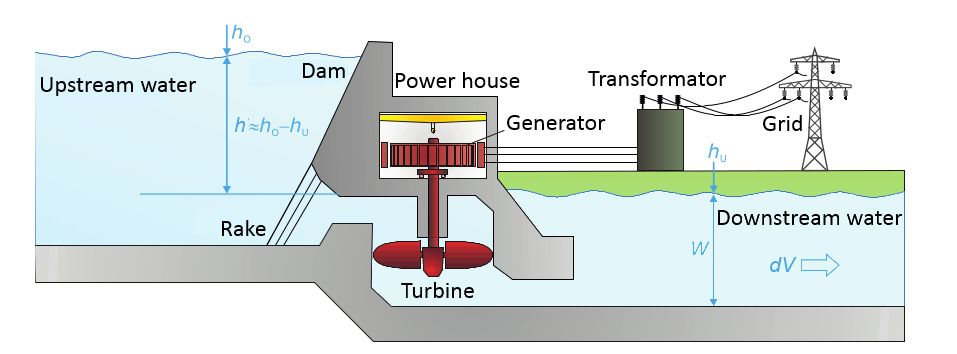
\includegraphics[width=15cm]{schema_hpp_en.png}
\caption[Schema of a run-of-the-river hydropower plant]{Schema of a run-of-the-river hydropower plant \cite{quaschning}}
\label{schema_hpp}
\end{figure}
\subsection{Output power}
A run-of-the-river power plant generates a power proportional to the water flow and the head, as seen in equation \ref{eq_power_1} \cite{quaschning}.
\begin{equation}
\label{eq_power_1} 
 P = \rho_\mathrm{water} \cdot g \cdot \dot{V}_\mathrm{turbine} \cdot h \cdot \eta_\mathrm{turbine} \cdot \eta_\mathrm{generator}
\end{equation}
With 
\begin{itemize}
\itemsep0em 
 \item $P$ \tabto{4cm} power produced by the generator \tabto{12cm} [\unit{W}]
 \item $\rho_\mathrm{water}$ \tabto{4cm} density of water \tabto{12cm} \unit[1000]{kg\textperiodcentered m\textsuperscript{-3}}
 \item $g$ \tabto{4cm} acceleration of gravity \tabto{12cm} \unit[9.81]{m\textperiodcentered s\textsuperscript{-2}}
 \item $\dot{V}_\mathrm{turbine}$ \tabto{4cm} water flow through the turbine \tabto{12cm} [\unit{m\textsuperscript{3}\textperiodcentered s\textsuperscript{-1}}]
 \item $h$ \tabto{4cm} head of water \tabto{12cm} [\unit{m}]
 \item $\eta_\mathrm{turbine}$ \tabto{4cm} efficiency of the turbine
 \item $\eta_\mathrm{generator}$ \tabto{4cm} efficiency of the generator
\end{itemize}


The head of water is the altitude difference between the surface of the river before and after the turbine. For run-of-the-river hydropower plants, it is assumed that the water level before the turbine is kept constant by the dam, while the water level downstream can vary. This happens when the water flow exceeds the capacity of the turbine and has to be deviated over the dam. With this assumption, the head of water is given by the equation \ref{eq_head}. The water flow in the turbine is at most \.{V}\textsubscript{n}, and an amount of residual water has to be substracted from the available water flow. The amount of residual water is fixed by law to ensure a minimum water flow in the rivers at all time, an is potentially incresed by the presence of a fish ladder or a passage for canoes. The water flow in the turbine by the equation \ref{eq_waterflow} \cite{quaschning}.
\begin{equation}
\label{eq_head} 
 h = h_\mathrm{n} +W_\mathrm{n}-W
\end{equation}
\begin{equation}
\label{eq_waterflow} 
 \dot{V}_\mathrm{turbine} = \min(\dot{V}_\mathrm{n},\dot{V}-\dot{V}_\mathrm{rest})
\end{equation}
Where $h_\mathrm{n}$, $W_\mathrm{n}$ and $\dot{V}_\mathrm{n}$ are respectively the nominal head, water level downstream from the dam and water flow, and W and \.{V} the real water level and water flow.
\newline
The  equation \ref{eq_power_1} becomes :
\begin{equation}
 \label{eq_power_2} 
 P = \rho_\mathrm{water} \cdot g \cdot \min(\dot{V}_\mathrm{n},\dot{V}-\dot{V}_\mathrm{rest}) \cdot (h_\mathrm{n} +W_\mathrm{n}-W) \cdot \eta_\mathrm{turbine} \cdot \eta_\mathrm{generator}
\end{equation}

\subsection{Types of turbines}

There are two families of water turbines : action turbines and reaction turbines. Action turbines use the kinetic energy of water, without any changes in pressure, while reaction turbines transform the potential energy of water into kinetic energy, decreasing the pressure. The main types of turbines for each family are \cite{quaschning} :
\begin{itemize}
 \item Action turbines
 \begin{itemize}
  \item Pelton turbine
  \item Turgo turbine
  \item Ossberger turbine or cross-flow turbines
 \end{itemize}
 \item Reaction turbines
 \begin{itemize}
  \item Kaplan turbines
  \item Bulb or tubular turbines
  \item Francis turbines
 \end{itemize}
\end{itemize}

The four types of turbines used for run-of-the-river plants are Pelton, Francis, Kaplan and crossflow. These turbines have optimal performances over ranges of water flow and hydraulic head : Kaplan turbine are appropriate for low-head plants, Francis for average heads and Pelton for low water flows and high heads.   

\subsection{Turbine and generator efficiencies}
\label{eff_turb_gen}
The efficiency of the turbine depends on the type of turbine and on the part-load range\cite{quaschning}\cite{pacer}. 

Figure \ref{efficiency_turb} gives the efficiency curves of different turbine types depending on the part load. These efficiencies can be approximated by the empiric function given in equation \ref{eq_eff} with the parameters given in table \ref{eff_param} \cite{quaschning}. In this equation, $\dot{V}_\mathrm{min}$ is the minimal water flow to start the turbine, $\dot{V}_\mathrm{n}$ is the nominal water flow of the turbine and $\dot{v}=\frac{\dot{V}-\dot{V}_\mathrm{min}}{\dot{V}_\mathrm{n}}$.

\begin{equation}
 \label{eq_eff}
\eta_\mathrm{T}= \left\{
    \begin{array}{ll}
	0 & \mbox{for } \dot{V} \leq \dot{V}_\mathrm{min}\\
        \frac{\dot{v}}{a_\mathrm{1}+a_\mathrm{2} \cdot \dot{v} + a_\mathrm{3} \cdot \dot{v}^2} & \mbox{for } \dot{V}_\mathrm{min}<\dot{V}<\dot{V}_\mathrm{n} \\
        \eta_\mathrm{T,n} & \mbox{for } \dot{V} \geq \dot{V}_\mathrm{n}
    \end{array}
\right.
\end{equation}


\begin{figure}[H]
\centering
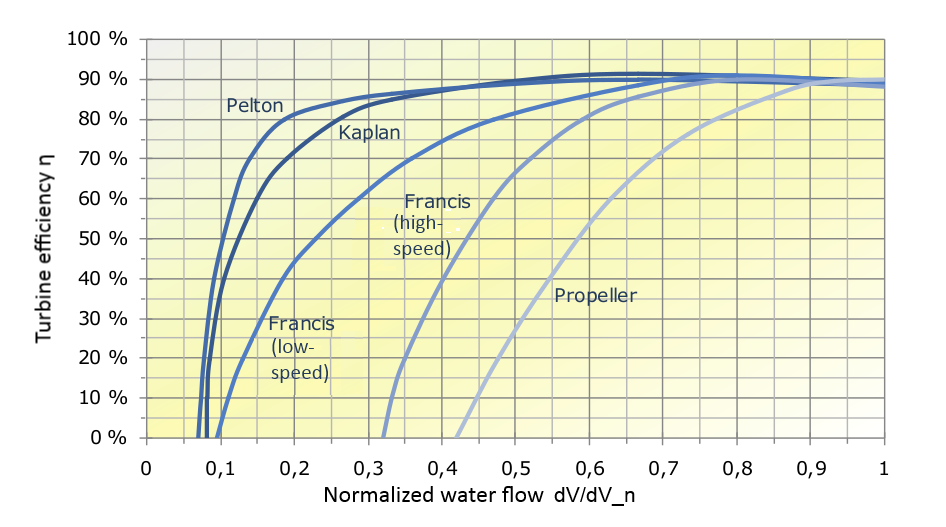
\includegraphics[width=12cm]{efficiency_turb_en.png}
\caption[Efficiency of different types of turbines depending on the part load ratio]{Efficiency of different types of turbines depending on the part load ratio (water flow / nominal water flow) \cite{raa89}}
\label{efficiency_turb}
\end{figure}


\begin{table}[H]
 \centering
 \caption[Parameters to calculate the turbine efficiency]{Parameters to calculate the turbine efficiency \cite{quaschning}}
 \label{eff_param}
 \begin{tabular}{|c|c|c|c|c|c|}
  \cline{2-6}
  \multicolumn{1}{c|}{}&$\dot{V}_\mathrm{min} / \dot{V}\mathrm{n}$ & $\eta_\mathrm{T,n}$& $a_\mathrm{1}$ & $a_\mathrm{2}$&$a_\mathrm{3}$ \\ 
  \hline
  Kaplan & 0.081& 0.895& 0.045 &0.965& 0.1 \\
  Pelton & 0.07& 0.885& 0.03& 0.99& 0.1\\
  Francis &0.095 &0.89 &0.18 &0.63 &0.31 \\
  Propeller &0.42 &0.9 &0.25 &0.28 &0.69\\
  \hline
 \end{tabular}
\end{table}

\label{sub:gen_eff}

The efficiency factor of the generator depends on its power and on the part-load range \cite{pacer}. The Swiss ``Bundesamt für Konjunkturfragen'' gives the values given in table \ref{eta_gen}.

\begin{table}[H]
 \centering
 \caption[Generator efficiency in full load and part load]{Generator efficiency in full load (left) and part load (right) \cite{pacer}}
 \label{eta_gen}
 \begin{tabular}{|C{3cm}|C{3cm}| C{1cm} |C{3cm}|C{3cm}|}
  \cline{1-2} \cline{4-5}
  $P_\mathrm{el} [kW]$ & $\eta_\mathrm{g,max}$  && $P_\mathrm{el}/P_\mathrm{el, max}$ & $\eta_\mathrm{g}/\eta_\mathrm{g,max}$ \\ 
  \cline{1-2} \cline{4-5}
  1 to 5 & \unit[80]{\%} to \unit[85]{\%} && 
  \multirow{4}{*}{\begin{tabular}{c}>\unit[50]{\%}\\\unit[25]{\%} \\\unit[10]{\%} \\\end{tabular}}& 
  \multirow{4}{*}{\begin{tabular}{c}\unit[100]{\%} \\\unit[95]{\%} \\\unit[85]{\%} \\\end{tabular}}\\
  5 to 20 & \unit[85]{\%} to \unit[90]{\%} &&& \\
  20 to 100 & \unit[90]{\%} to \unit[95]{\%} &&&\\ 
  More than 100 & \unit[95]{\%} &&&\\ 
  \cline{1-2} \cline{4-5}
\end{tabular}
\end{table}

\section{Existing models and approaches}

Several hydropower models have been or are being developed, among which : 
\begin{itemize}
 \item The r.green.hydro model, developed by EURAC Research in Bolzano \cite{grass} to work with the GRASS GIS software computes hydropower potential from discharge raster maps with theoretical, legal, technical, ecological or economic constraints.
 \item The simple{\_}hydropower{\_}model from James Sample \cite{sample} estimates the potential impacts of climate change on Scotland's run-of-river hydropower potential. It takes historical and future flow data as input, a user-defined head of water, and set the nominal water flow based on the flow duration curve, and computes the output.
 \item The OSeMOSYS community \cite{osemosys} developed a browser-based open source interface for energy systems modeling which includes hydropower.
 \item The renpass model \cite{wiese} developed by Frauke Wiese is another energy systems modeling tool with a hydropower part developed by Gesine Boekenkamp \cite{gesine}. It uses a mathematical approach to assess the production, based on the capacity utilization of previous years and the water level variations.
 \item Matthias Stark calculated the production from German hydropower in his PhD work, by approximated the nominal water flow of a plant with the mean annual water flow of the river \cite{stark}.
\end{itemize}
The objective of this work was not to asses hydropower potential but rather to develop a model capable of producing feed-in time series of existing plants. The above-mentioned works were reviewed and some similar approaches were used to develop a model compliant with the expectations of the Reiner Lemoine Institute and the openFRED project.
	\chapter{Data basis}
\label{chap:data_basis}

The previous chapter mentioned parameters affecting hydroelectricity production. In this chapter, the data sets available for this work will be described and analyzed. This include power plants data registers and production data, as well as runoff data sets. 

\section{Hydroelectricity}
\label{sec:db_hydroelec}
In order to simulate the hydroelectricity production of a region, a register of all existing power plants is needed. The simulated hydroelectricity production should then be compared to real production data, in order to validate the model. This process can only be consistent if the actual production data comes from the same plants listed in the power plants register. This section presents the available data sets for existing plants and production, and shows the significant discrepancies between them. 

\subsection{Open Energy Database}
\label{sub:hpp_reg}
This work, as well as the project open\_FRED, is linked to the OpenEnergy Platform, developed within the open\_eGo project. The OpenEnergy Platform, through the OpenEnergy Database, provides necessary tools for transparent and collaborative energy system modeling \cite{oedb}, such as grid data, power plants register, geography data or weather data. The power plant register was extracted from the Open Power System Data (OPSD) and has 7491 entries for run-of-the-river hydropower plants and 5 entries for reservoir plants in Germany. The run-of-the-river entries contain, among others, the following information :
\begin{itemize}
\itemsep-0.5em 
 \item Company operating the plant and network operator information
 \item Adress and state
 \item Startup, retrofit and shutdown years
 \item Electrical capacity [\unit{MW}]
 \item Position (latitude, longitude, and GIS geometry)
\end{itemize}

Figure \ref{oedb_capa} shows the repartition of the capacity of OPSD run-of-the-river and reservoir plants. This is consistent with the Umweltbundesamt numbers of 6500 to 7500 hydropower plants excluding pumped hydro, among which 406 with a nominal power above \unit[1]{MW} \cite{uba_wasserkraft}. The OPSD also has entries for pumped storage plants, listed in Tab. \ref{oedb_pump}.

\begin{figure}[H]
\centering
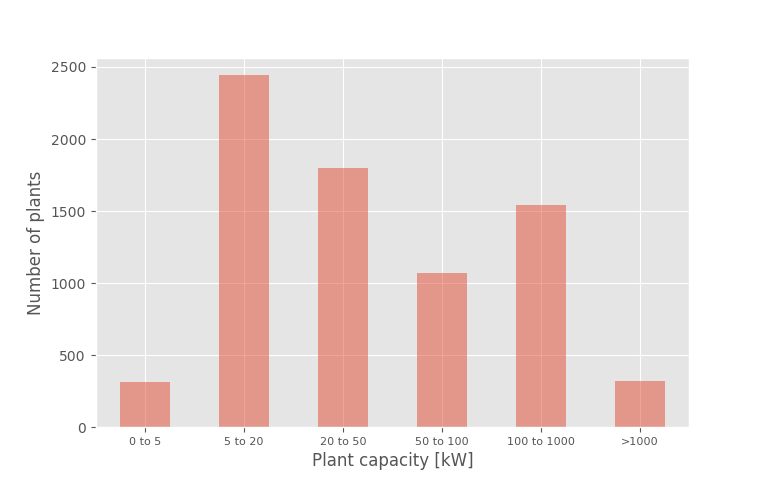
\includegraphics[width=10cm]{oedb_capa.png}
\caption[Repartition of the capacity of run-of-the-river and reservoir plants in the Open Power System Data]{Repartition of the capacity of run-of-the-river plants plants in the Open Power System Data}
\label{oedb_capa}
\end{figure}

\begin{table} [H]
\footnotesize
  \centering
  \caption[Number of pumped storage plants and installed capacity per federal state]{Number of pumped storage plants and installed capacity per federal state \cite{oedb}}
  \label{oedb_pump}
  \begin{tabular}{|c|cc| }
  \hline
  \textbf{State} & Number 	& 	Capacity [\unit{MW}] 	\\
  \hline
  SH	&	3	&	119.1	\\
  NI	&	1	&	220	\\
  NRW	&	2	&	291	\\
  HE	&	2	&	623	\\
  BW	&	7	&	1873	\\	
  BY	&	7	&	587	\\
  SN	&	8	&	1085	\\
  ST	&	2	&	79.7	\\
  TH	&	16	&	1509.4	\\
  \hline
  \end{tabular}
\end{table}

\subsection{Comparison with the Agentur für Erneuerbare Energie data}
\label{sub:prod_data}

A simulation based on the OPSD register should be compared with real production data, to assess the precision of the model.\newline The hydroelectricity production of Germany is calculated by the Bundesverband der Energie- und Wasserwirtschaft (BDEW), a federal organisation of companies in the sector of water and energy, and published by the Agentur für Erneuerbare Energien (AEE). The AEE provides data about the installed capacity, electricity generation over the year, and number of hydropower plants for each federal state from 2001 to 2014 \cite{aee}. This data contains run-of-the-river and reservoir plants, as well as pumped storage power plants with natural inflow for which only the production from natural inflow is accounted for. There is therefore no consistent way of comparing it with the OPSD data because the OPSD does not state which part of the capacity of pumped hydro plants uses natural inflow. \newline
Table \ref{oedb_aee_diff} lists the number of plants and installed capacity per federal state from the OPSD (run-of-the-river and reservoirs) and the AEE, as well as the relative difference for each state, with the AEE data as reference. It shows that even in states with no pumped storage facilities, such as Rhineland-Palatinate, these two sources give very different values for the numbers of plants and installed capacities. \newline
The relative difference is shown on figures \ref{map_diff_num} and \ref{map_diff_pow}, which respectively display the differences in the number of plants and in the installed capacity. The analysis of these two maps and of Tab. \ref{oedb_aee_diff} shows that the OPSD and AEE data sets seem to be consistent in three federal states : Thuringia, Saxony-Anhalt and Mecklenburg-Vorpommern (Berlin and Bremen being excluded due to the near absence of hydropower). The discrepancies in other federal states can be explained by different reasons. First, the data of the the AEE are based on run-of-the-river plants, reservoir plants and natural inflow in pumped storage plants, while the data from the OPSD shown here only account for run-of-the-river and reservoir plants (the pumped hydro plants having been excluded due to the lack of information on the presence of natural inflow). Moreover, the OPSD register of reservoir plants, with its five entries, is clearly incomplete. This is why both the number of plants and the installed capacity are greater in the AEE data for most states. Second, the pumped storage and reservoir plants tend to have a bigger capacity than most run-of-the-river plants, which explains that the difference in installed capacity is not proportional to the difference in number of plants. Finally, rivers often mark boundaries between states and countries, and some hydropower plant are operated by two countries or inject electricity into the grid of a neighboring country. It is possible that the AEE and the OPSD do not count the installed capacity in the same manner in this situation.

\begin{table}[H]
\footnotesize 
 \centering
 \caption[Number of hydropower plants and installed capacity per federal state]{Number of hydropower plants and installed capacity per federal state}
 \label{oedb_aee_diff}
 \begin{tabular}{|c|cc|cc| cc|}
  \cline{2-7}
  \multicolumn{0}{c|}{} &\multicolumn{2}{c}{\textbf{OPSD \cite{oedb}}}&\multicolumn{2}{|c|}{\textbf{AEE \cite{aee}}}&\multicolumn{2}{c|}{\textbf{Difference}} \\
  \hline
  \textbf{State} & Number 	& 	Capacity [\unit{MW}] 	&	Number 	& 	Capacity [\unit{MW}] 	&	Number [\unit{\%}] 	&	Capacity [\unit{\%}] \\
  \hline
  SH	&	29	&	8.1		&	24	&	5		&	20.8		&	62.8	\\
  HH	&	1	&	0.11		&	1	&	0.1		&	0		&	10	\\
  NI	&	258	&	56.3		&	257	&	70		&	0.4		&	-19	\\
  HB	&	1	&	10		&	1	&	10		&	0		&	0	\\
  NRW	&	438	&	152.8		&	409	&	202		&	7.1		&	-24.3	\\
  HE	&	465	&	91.9		&	482	&	82		&	-3.5		&	12.1	\\
  RLP	&	217	&	40.8		&	199	&	218		&	9		&	-81.3	\\
  BW	&	1741	&	464.5		&	1485	&	960		&	17		&	-51.6	\\	
  BY	&	3659	&	835.7		&	3578	&	2661		&	2.3		&	-68.6	\\
  SL	&	26	&	11.1		&	26	&	24		&	0		&	-53.6	\\
  B	&	0	&	0		&	0	&	0		&	0		&	0	\\
  BB	&	42	&	5.3		&	38	&	6		&	10.5		&	-11.8	\\
  MV	&	25	&	3		&	24	&	3		&	4.2		&	-0.1	\\
  SN	&	322	&	134.4		&	330	&	99		&	-2.4		&	35.8	\\
  ST	&	57	&	26		&	52	&	26		&	9.6		&	0.2	\\
  TH	&	205	&	32.6		&	198	&	32		&	3		&	2	\\
  \hline
 \end{tabular} 
\end{table}


\begin{figure}[H]
\centering
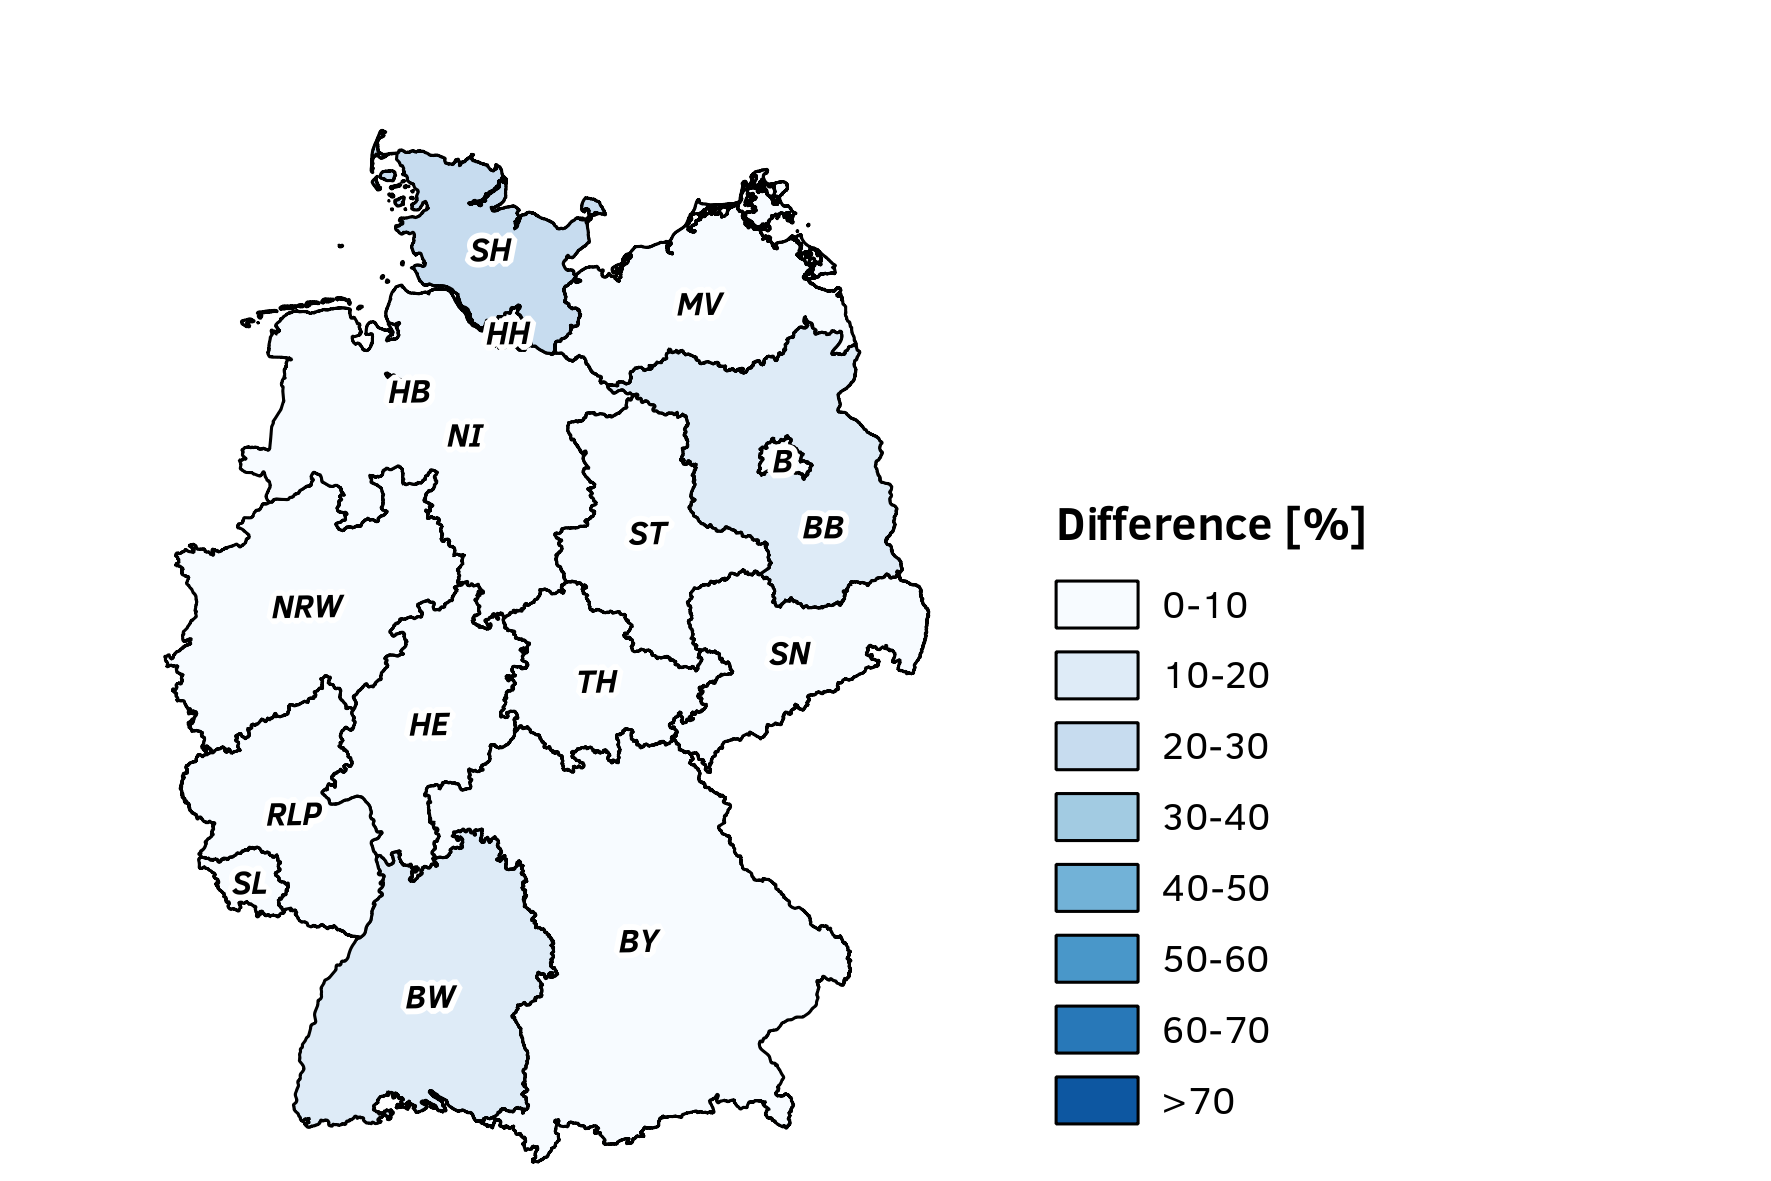
\includegraphics[width=13cm]{map_diff_num.png}
\caption[Absolute difference in the number of plants between OPSD and AEE]{Absolute difference in the number of plants between OPSD and AEE}
\label{map_diff_num}
\end{figure}


\begin{figure}[H]
\centering
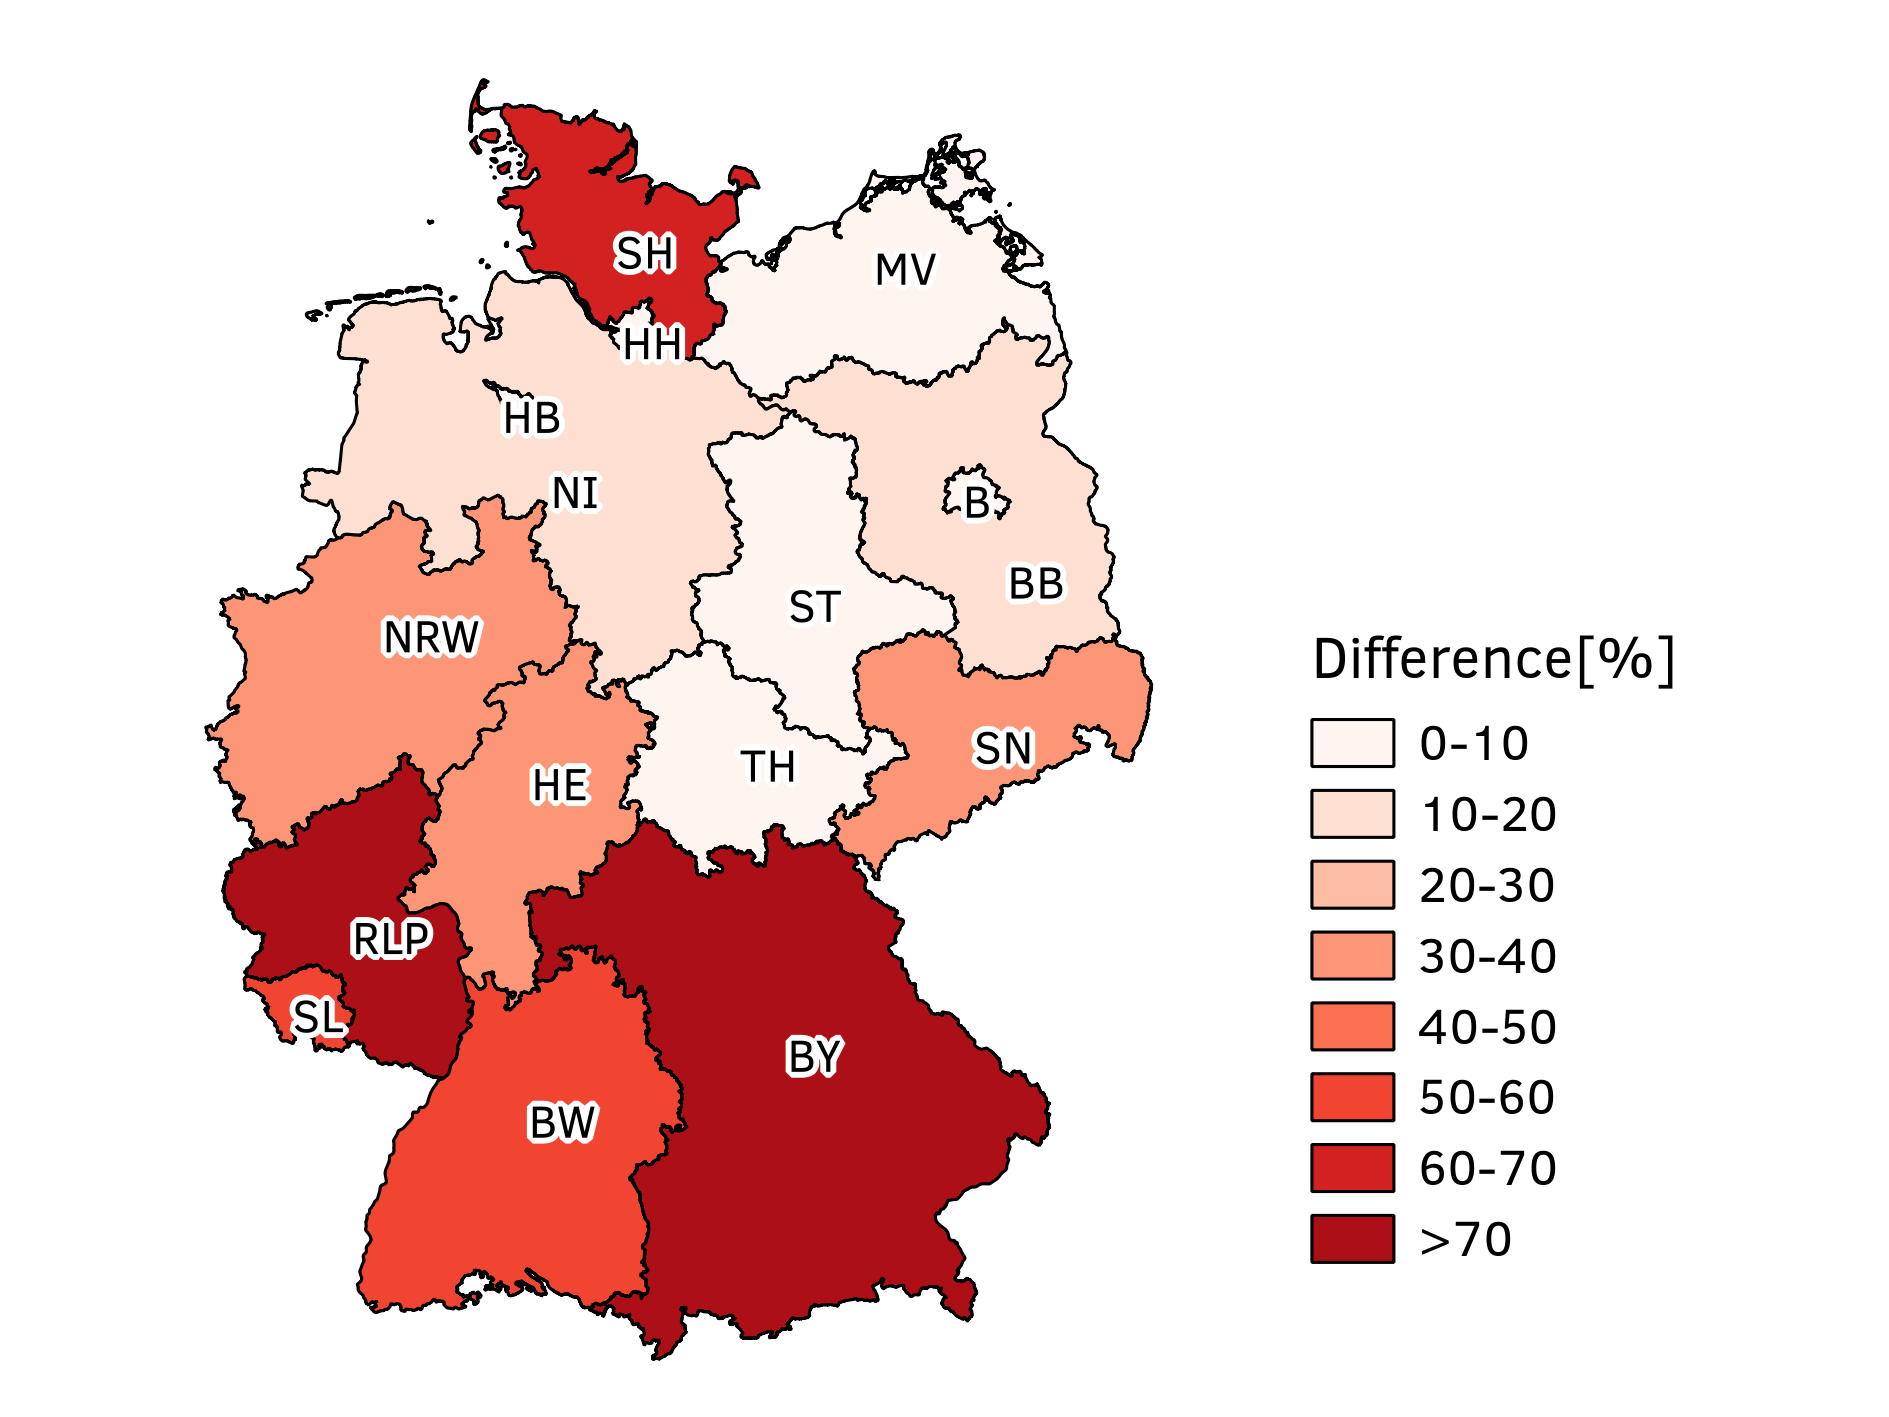
\includegraphics[width=13cm]{map_diff_pow.png}
\caption[Absolute difference in the installed capacity between OPSD and AEE]{Absolute difference in the installed capacity between OPSD and AEE}
\label{map_diff_pow}
\end{figure}


\subsection{Future data set}

The german Bundesnetzagentur is developing a register of every energy production facility in Germany, called ``Marktstammdatenregister''. This register should give a complete overview of the power plants in Germany, sorted by energy carrier and type of plant (reservoir, run-of-the-river, pumped hydro...), and listing the location and nominal power, as well as the presence or not of a restriction of the usable water flow due to a fish ladder or fish protection system for instance \cite{MaStR}. \newline
When published, it will be uploaded in the OEDB and will provide a more consistent data set of existing plants.

\section{Runoff data - measured}

\label{sec:meas_runoff}

In order to study rivers, 

Water levels and water flows of the main rivers are regularly measured and documented by several organizations, in order to keep track of the history of the waterways and to anticipate potential floods. Measurement stations have been installed and monitored for decades, dating back as far as 1816 for Germany, and the time series are stored in databases. There are different ways to measure the water flow, such as propeller gauges, ultrasonic flow meter, or acoustic current profilers. In Germany there are around 4300 stations measuring water flow or water level, operated by different stakeholders \cite{bafg_hyd}.  The German Federal Institute of Hydrology (Bundesanstalt für Gewässerkunde – BfG) is a supreme federal agency within the portfolio of the Federal Ministry of Transport and Digital Infrastructure. As such it is the federal government's scientific institution for research, assessments, and consulting in the fields of hydrology, uses, quality and conservation of waters and ecology \cite{bafg}. The BfG gathers data about water levels and water flows since its founding in 1949 and publishes it every year in the ``Deutsches Gewässerkundliches Jahrbuch'' (DGJ). The BfG also operates the HYDABA database, in which times series for water flow and water level are stored, going back to 1816 for daily values and 1981 for hourly values. This database gathers water levels from around 600 gauges and water flows from around 250 stations, operated by the Federal Waterways and Shipping Administration (WSV). The data from the HYDABA database can be provided to, among others, universities, public administrations, engineering or insurance companies \cite{bafg_hyd}. \newline
The WSV, through its service Pegelonline, publishes raw values of water levels from its gauge stations in Germany over the previous 30 days. Some of the stations also measure water flows \cite{pegelonline}. The locations of the gauges are shown on Fig. \ref{pegelonline}.

\begin{figure}[H]
\centering
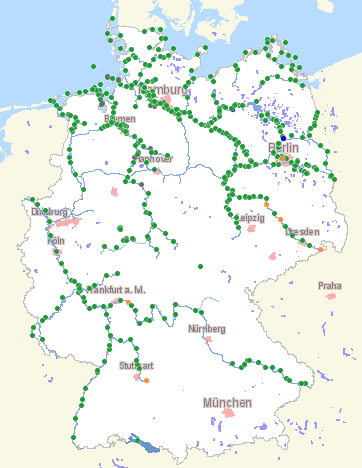
\includegraphics[width=8cm]{pegelonline.png}
\caption[Locations of the gauge stations]{Locations of the gauge stations \cite{pegelonline}}
\label{pegelonline}
\end{figure}

Another source for runoff data is the Global Runoff Data Center (GRDC, 56068 Koblenz, Germany) which operates, on a non-profit basis, a world-wide database of measured runoffs. The GRDC can transfer its data on demand and under certain conditions (according to its policy guidelines for the dissemination of data).\newline

Other countries have similar databases for measured river data. In France, the ``Banque Hydro'' is run by the SCHAPI (Service Central d'Hydrométéorologie et d'Appui à la Prévision des Inondations), a section of the french Ministry of Ecology, Sustainable Development and Energy, and gathers and publishes data from around 5000 gauge stations.

\section{Runoff data - modeled}

\label{sec:mod_runoff}
Modeling runoff is a difficult task, as the model has to assess the interactions between river sources, relief, rainfall, local soil and vegetation type, as well as anthropogenic use. This can be done using GIS \cite{bayazit}, by assigning each cell with the precedent parameters. The water input in each cell (rainfall, water sources and runoff from other cells) is converted in runoff from the cell by subtracting the water lost by infiltration, evapotranspiration, or anthropogenic use, and the runoff direction is given by the slope, calculated using a digital elevation model \cite{heywood}. \newline
The WaterGAP software, developed by the universities of Kassel and Frankfurt, uses this method to calculate flows and reservoirs of water around the globe, as shown on Fig. \ref{waterGAP}.
\begin{figure}[H]
\centering
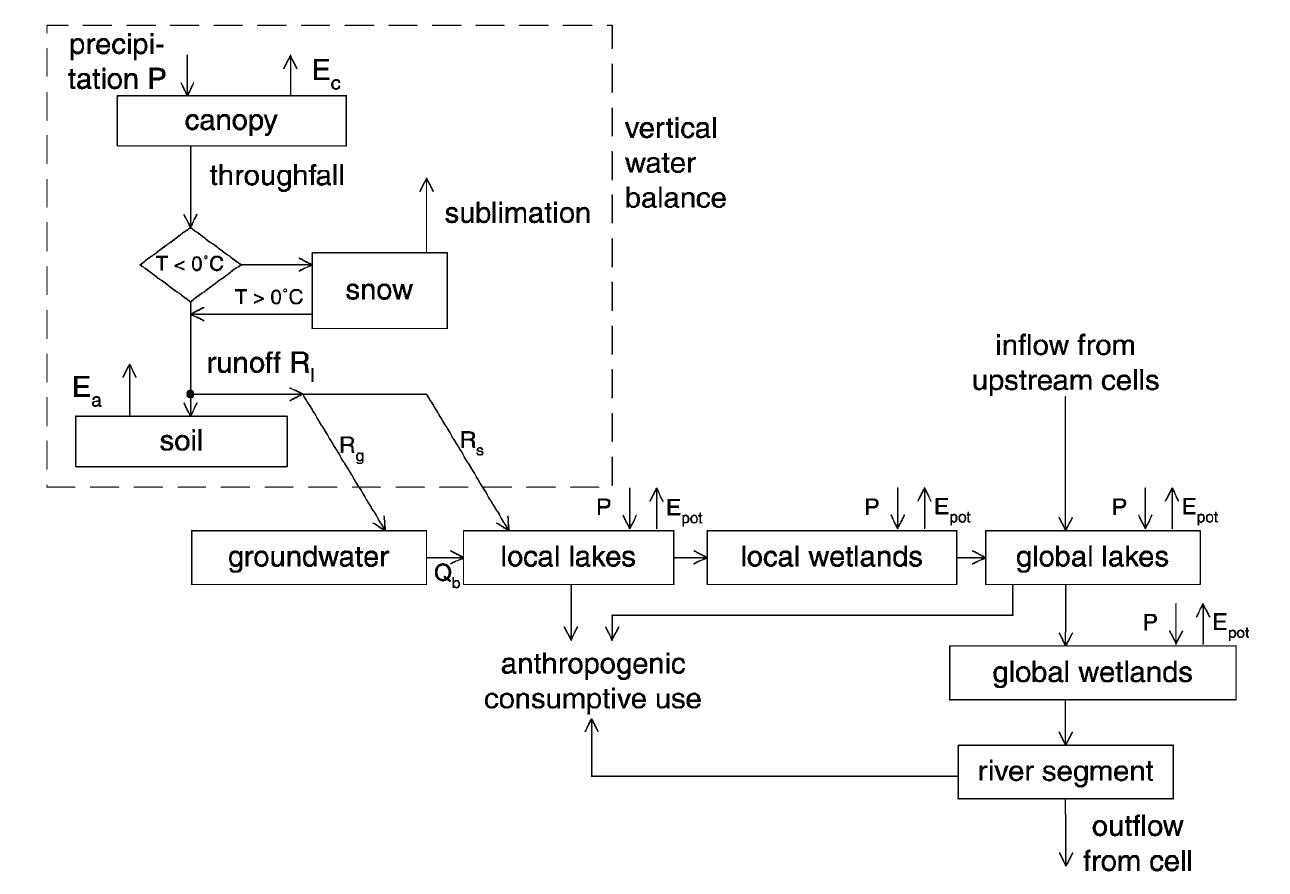
\includegraphics[width=15cm]{waterGAP.png}
\caption[Representation of a global hydrological from the WaterGAP software]{Representation of a global hydrological from the WaterGAP software \cite{doll}}
\label{waterGAP}
\end{figure}
Other runoff models exist, for example the WEAP model of the Stockholm Environment Institute \cite{weap}, the HYPE model developed by the Swedish Meteorological and Hydrological Institute \cite{hype}, or the TOPKAPI model of PROGEA \cite{topkapi}. \newline
Given that this work is part of the openFRED project (see Ch. \ref{chap:introduction}), the runoff data should eventually be accessible from open source databases or software. The weather aspects of the openFRED project are handled together with the Helmholtz Zentrum Geesthacht : the weather model COSMO is being adapted the the requirements of the project, and, when ready, will deliver the input data (rainfall, temperature, ...) for an existing open source runoff model. \newline
In the meantime, modeled time series from the WaterGAP software were used in this work. The data takes the form of a raster with a resolution of 5 angular minutes, each raster cell containing time series of runoff with a daily temporal resolution, from 2006 to 2009. When only the cells with an average runoff over \unit[100]{m\textsuperscript{3}\textperiodcentered s\textsuperscript{-1}} are displayed, the German river system is recognizable and the cells overlap the layout of Germany main rivers from the Digital Landscape Model \cite{dlm250} (see Fig. \ref{map_watergap_dlm}).

\begin{figure}[H]
\centering
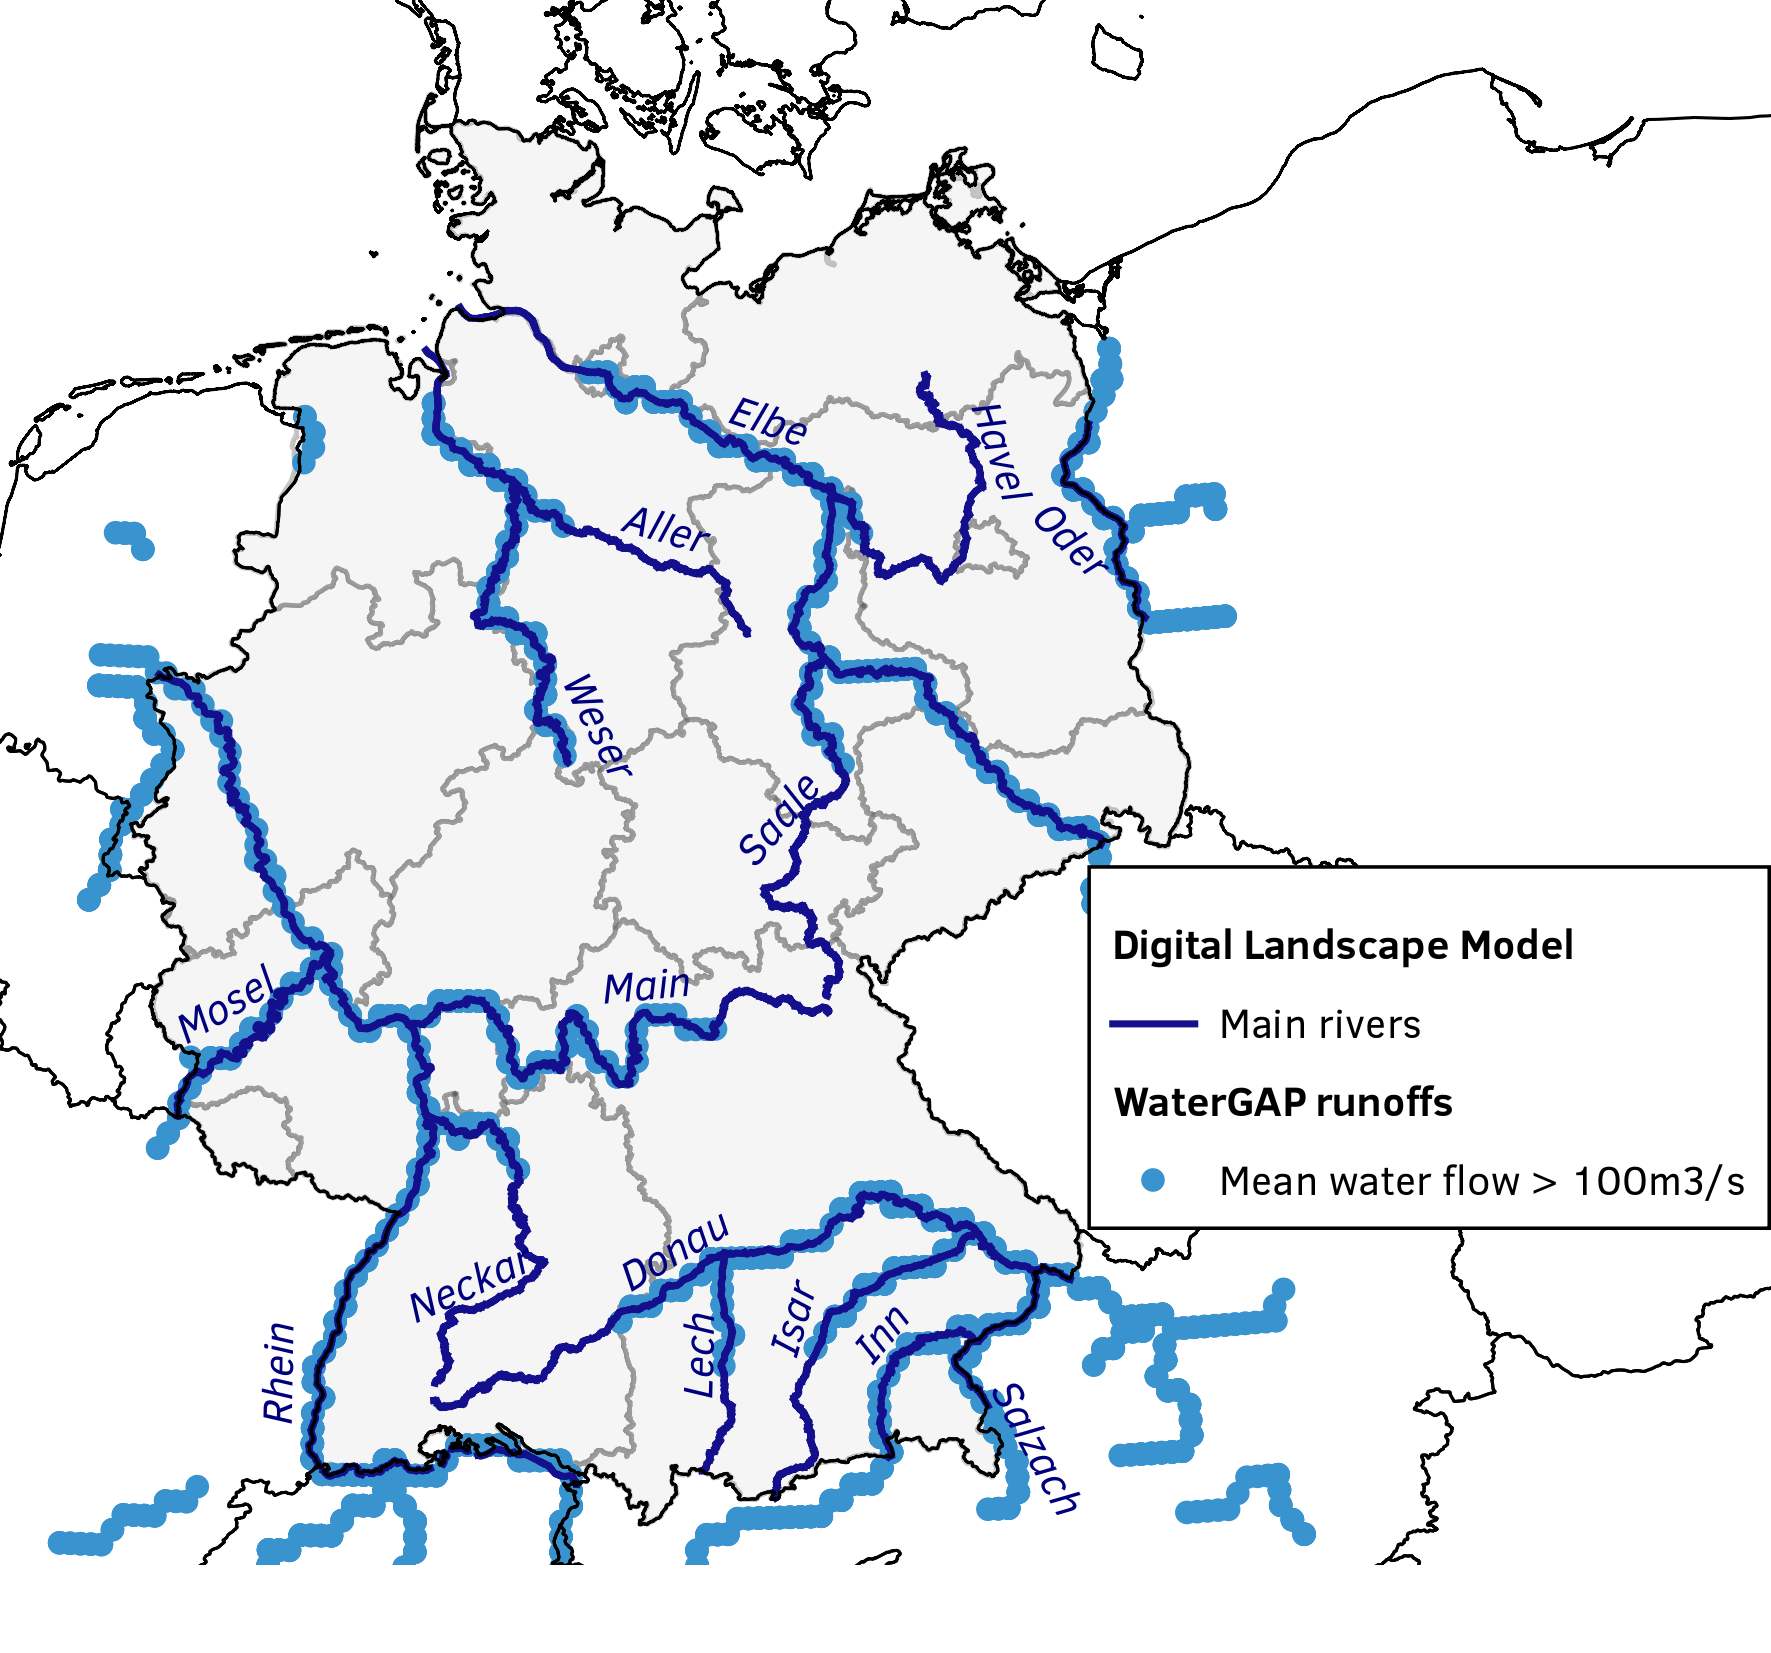
\includegraphics[width=13cm]{map_watergap_dlm.png}
\caption[Representation of the German main rivers from waterGAP and DLM]{Representation of the German main rivers from waterGAP and DLM}
\label{map_watergap_dlm}
\end{figure}

	\chapter{Methodology}
\label{chap:methodology}

\section{Developement of the simulation model}
\subsection{Specifications}
In order to predict with precision the electrical output of a run-of-the-river power plant, the following parameters and values would be needed : 
\begin{itemize}
\itemsep0em
 \item Power plant parameters : 
 \begin{itemize}
  \item nominal water flow through the turbine ($Q_\mathrm{nenn}$)
  \item nominal head of water ($H_\mathrm{nenn}$)
  \item nominal water level ($W_\mathrm{nenn}$)
  \item efficiency curve of the turbine ($\eta_\mathrm{turbine}$) 
  \item efficiency of the generator ($\eta_\mathrm{generator}$)  
  \item unusable water flow ($Q_\mathrm{rest}$)  
 \end{itemize}
 \item Input time series : 
 \begin{itemize}
  \item actual water flow through the turbine ($Q$)
  \item actual water level downstream from the turbine ($W$)
 \end{itemize}
\end{itemize}

However, if such precise data can be found for single power plants, it is not easily accessible at a state or country-wide level. The OEDB database lists the location and nominal power of the plants, without further information on their design. The german Bundesnetzagentur is developing a register of every energy production facility in Germany, called MaStR (Marktstammdatenregister). This register should give a complete overview of the power plants in Germany, sorted by energy carrier and type of plant (reservoir, run-of-the-river, pumped hydro...), and listing the location and nominal power, as well as the presence or not of a restriction of the usable water flow due to a fish ladder or fish protection system for instance \cite{MaStR}. This last information is not yet available in registers such as the OEDB.\newline
Therefore, the model should be able to extrapolate missing data and to make some assumptions when optional input parameters are not provided. The only compulsory input parameter will be the broadly available nominal power of the turbine and section \ref{missing_data} explains how other parameters can be assumed or extrapolated. \newline
In terms of time series, in addition to the water flow over the simulated period, the model will take as input the water flow over several years in order to extrapolate missing parameters. Section \ref{rel_river_data} will go more in details into the reasons why water level data is not relevant. \\
The desired outputs for the model are electricity production time series per power plant or per area. It should also be possible to simulate several plants in one go.

\subsection{Collection and administration of data basis}

It is estimated that among the 6500 to 7500 hydropower plants in Germany, only 406 have a nominal power above 1MW \cite{uba_wasserkraft}. Out of 7500 run-of-the-river hydropower plants in the OpenEnergy Database, 5600 have a capacity under 100kW (see figure \ref{oedb_capa} in section \ref{hpp_register}).  However, the plants under 1MW account for a small part of the total installed power (see figure \ref{uba_hpp}). For that reason, the generator efficiency has been approximated to 95\% for all power plants is this work.

\begin{figure}[H]
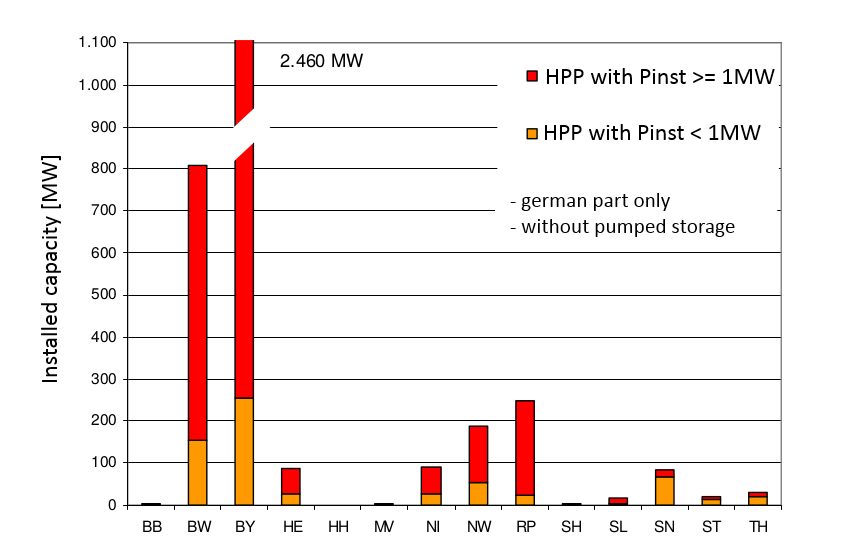
\includegraphics[width=15cm]{uba_hpp_en.png}
\caption[Installed power pro Bundesland for plants over and under 1MW]{Installed power pro Bundesland for plants over and under 1MW \cite{uba_wasserkraft}}
\centering
\label{uba_hpp}
\end{figure}
XXX take some from above and complete : inputs, parameters and validation data
XXX write here the stuff about W not being relevant

For this reason, the state-wide simulation of hydropower production presented in the case study from section XXX UPDATE WHEN READY XXX as been conducted for XXX TH or ST or MV XXX, in order to compare the results of the simulation based on the OEDB register with the yearly production values given by the AEE.

In this work, data from the BfG was used as input to test the model (XXX put references of teil über Mosel und Thuringe XXX), as well as data from the french ``Banque Hydro'' (XXX reference of the teil über Hydroraon XXX). The ``Banque Hydro'' is run by the SCHAPI (Service Central d'Hydrométéorologie et d'Appui à la Prévision des Inondations), a section of the french Ministry of Ecology, Sustainable Development and Energy, and gathers data from around 5000 gauge stations.


\subsection{Simulation results and evaluation}
XXX Over which period of time, stepsize, error...

\section{Data preprocessing}

\subsection{Power plants register - OEDB}
XXX GIS/SQL code from Ludwig. Next neighbour finden, gauge station has to be on the same river...
\subsection{Runoff data}
XXX structure in DB

\section{Simulation}

\section{Evaluation of results}


	\chapter{Simulation model}
\label{chap:simulation_model}

\section{General structure}

\subsection{Classes of the model}
The model is developed in Python and consists of two classes (see Fig. \ref{uml}) : the HydropowerPlant class, which represents a run-of-the-river power plant and the Modelchain class which represents the simulation of one plant. The attributes and methods of each class are detailled in Tab. \ref{att_meth}. \newline
A Modelchain object takes a HydropowerPlant object as input, as well as runoff time series. If attributes from the HydropowerPlant object are missing, the Modelchain object calculates them during initialization, through the extrapolation processes presented in Sec. \ref{sub:assumptions}. The implementation of this process is detailed in Sec. \ref{sub:check_feas} to \ref{sub:get_type}.
\begin{figure}[H]
\centering
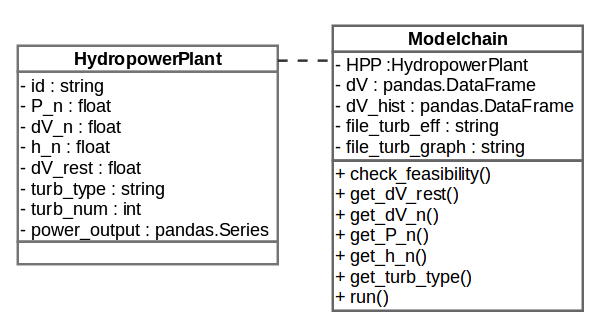
\includegraphics[width=12cm]{uml.png}
\caption{Classes of the hydropower model}
\label{uml}
\end{figure}

\begin{table}
\footnotesize
 \centering
 \caption{Attributes and methods of the classes}
 \label{att_meth}
 \begin{tabular}{|l|l|l|p{6cm}|}
  \cline{2-4}
  \multicolumn{1}{c|}{}&\multicolumn{3}{c|}{\textbf{class HydropowerPlant}}\\ \hline
  \multirow{8}{*}{\rotatebox[origin=c]{90}{\textbf{Attributes}}}&id&string&Identification of the plant\\
  &P{\_}n&float&Nominal power of the plant in \unit{W}\\
  &dV{\_}n&float&Nominal inflow of the plant in \unit{m\textsuperscript{3}\textperiodcentered s\textsuperscript{-1}}\\
  &h{\_}n&float&Nominal head of water in \unit{m}\\
  &dV{\_}res&float&Residual water flow in \unit{m\textsuperscript{3}\textperiodcentered s\textsuperscript{-1}}\\
  &turb{\_}type&string&Type of turbine(s)\\
  &turb{\_}num&int&Number of turbines. Default : 1\\
  &power{\_}output&pandas.Series&Power output in \unit{W}\\
  \hline
  \multicolumn{4}{c}{}\\
  \cline{2-4}
  \multicolumn{1}{c|}{}&\multicolumn{3}{c|}{\textbf{class Modelchain}}\\ \hline
  \multirow{5}{*}[-1cm]{\rotatebox[origin=c]{90}{\textbf{Attributes}}}&HPP&HydropowerPlant&Plant to simulate\\
  &dV&pandas.DataFrame&Runoff time series in \unit{m\textsuperscript{3}\textperiodcentered s\textsuperscript{-1}} with DateTime index over the period to simulate\\
  &dV{\_}hist&pandas.DataFrame&Runoff time series in \unit{m\textsuperscript{3}\textperiodcentered s\textsuperscript{-1}} with DateTime index over several past years\\
  &file{\_}turb{\_}eff&string&File containing parameters about turbine efficiencies\\
  &file{\_}turb{\_}graph&string&File containing the characteristic diagrams\\
  \hline
  \multirow{7}[5]{*}{\rotatebox[origin=c]{90}{\textbf{Methods}}}&check{\_}inputs()&boolean&Checks if input data is sufficient \\
  &get{\_}dV{\_}res()&float&Calculates residual runoff in \unit{m\textsuperscript{3}\textperiodcentered s\textsuperscript{-1}}\\
  &get{\_}dV{\_}n()&float&Calculates nominal runoff in \unit{m\textsuperscript{3}\textperiodcentered s\textsuperscript{-1}}\\
  &get{\_}P{\_}n()&float&Calculates nominal power in \unit{W}\\
  &get{\_}h{\_}n()&float&Calculates nominal head in \unit{m}\\
  &get{\_}turb{\_}type()&string&Finds type of turbine\\
  &run{\_}model()&void&Calculates HPP.power{\_}output in \unit{W}\\
  \hline
 \end{tabular}
\end{table}

\subsection{Inputs and outputs}

The HydropowerPlant class has one compulsory parameter (id) and six optional parameters (P{\_}n, dV{\_}n, h{\_}n, dV{\_}res, turb{\_}type, turb{\_}num). The number of turbines (turb{\_}num) is by default set to one when not filled in and the other optional parameters are extrapolated in the Modelchain class. \newline 
The Modelchain class takes pandas DataFrames as input for runoff. They can be read from csv files or extracted from a database, as presented in Sec. \ref{sub:ex_with_csv} and \ref{sub:ex_with_oedb}. These DataFrames require a DateTime index and a column named 'dV' containing runoff values. In order to correctly extrapolate the nominal water flow and the residual water flow from the historic values, DataFrame 'dV{\_}hist' has to cover many years (10 to 25 according to \cite{pacer} and \cite{cetmef}). Moreover, the time series should preferably be of whole years to avoid errors due to seasonal changes. \newline
The output power in \unit{W} is stored in the power{\_}output attribute of the HydropowerPlant object, as a pandas Series with the same DateTime index as the input 'dV' DataFrame.

\section{Implementation details}

\subsection{Initialization of Modelchain class}

When a Modelchain object is created, an initialization process takes place to check the integrity of the input and, if needs be, extrapolate the missing input data. The initialization process is presented in Fig. \ref{init} and the different methods are detailed in the following sections.

\begin{figure}[H]
\centering
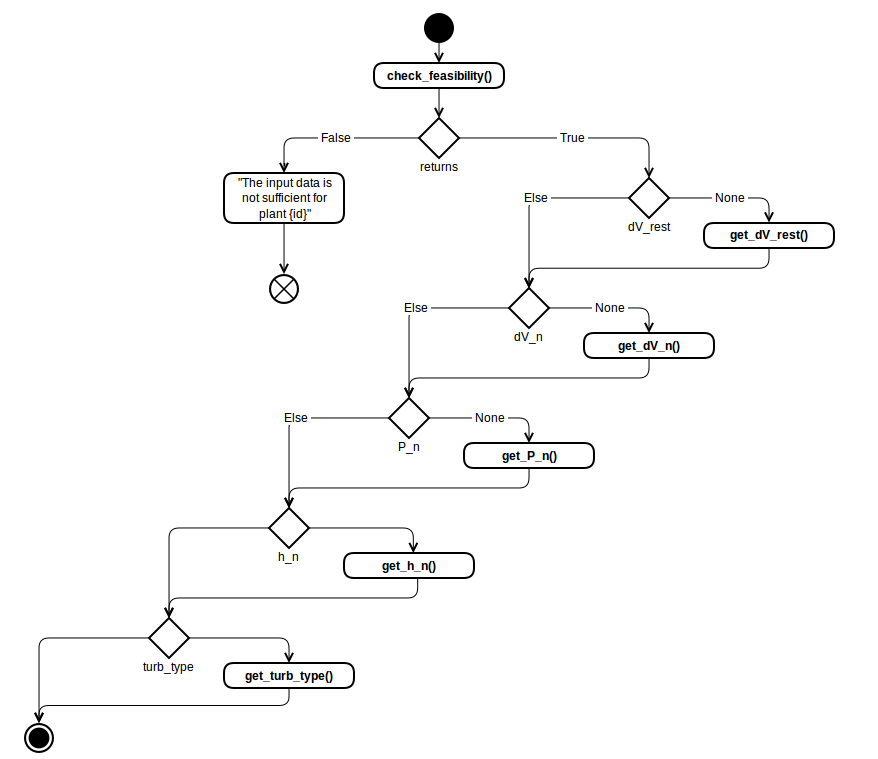
\includegraphics[width=15cm]{init.png}
\caption{Initialization of Modelchain class}
\label{init}
\end{figure}

\subsection{Method check{\_}inputs()}
\label{sub:check_feas}

When a Modelchain object is initialized, the missing parameters of the HydropowerPlant object are extrapolated from the known parameters and the runoff history. For the extrapolation to be possible, enough parameters have to be filled in. With two parameters among  P{\_}n, dV{\_}n and h{\_}n can the third be calculated using the power equation in nominal operation (Eq. \eqref{eq_nom}) with nominal efficiencies of the generator and the turbine approximated to respectively \unit[95]{\%} and \unit[90]{\%}. If the runoff history is filled in, it can be use to extrapolate the nominal and residual water flows. If it is not filled in, the residual water flow can be set to 0 as it is very small part of the actual water flow. The type of turbine is then extrapolated from the nominal head and water flow.
\begin{equation}
\label{eq_nom} 
 P_\mathrm{n} = \rho_\mathrm{water} \cdot g \cdot \dot{V}_\mathrm{n} \cdot h_\mathrm{n} \cdot \eta_\mathrm{turbine, n} \cdot \eta_\mathrm{generator, n}
\end{equation}

Therefore, the first step of the initialization is to check the feasibility of the simulation. This is done with a logical test on the presence of inputs. The logical expression, obtained by filling in a Karnaugh map (see Fig. \ref{karnaugh}), is given in Eq. \eqref{eq_feas}.

\begin{equation}
\label{eq_feas} 
 Feasibility = (h_\mathrm{n} \land P_\mathrm{n}) \lor ((h_\mathrm{n} \lor P_\mathrm{n}) \land (\dot{V}_\mathrm{hist} \lor \dot{V}_\mathrm{n}))
\end{equation}

\begin{figure}[H]
\centering
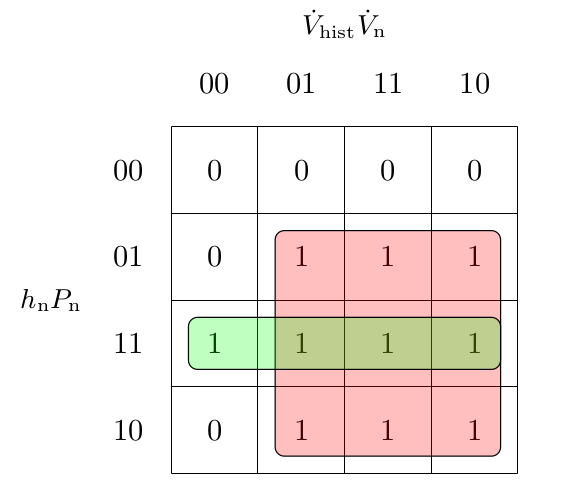
\includegraphics[width=8cm]{karnaugh.png}
\caption{Karnaugh map of simulation feasibility depending on inputs}
\label{karnaugh}
\end{figure}

\subsection{Method get{\_}dV{\_}res()}
\label{sub:getdVres}
The approach chosen to calculate the residual water flow is given in Sec. \ref{sub:assumptions}. It is implemented in the model within the get{\_}dV{\_}res() method of the Modelchain class, called during initialization.\newline If no runoff history has been specified, the residual water flow is set to zero. Otherwise, the ten most recent years of the runoff history are aggregated in a mean flow duration curve from which \.{V}\textsubscript{347} is extracted as the water flow attained or exceeded 347 days a year. The residual water flow \.{V}\textsubscript{res} is then calculated following Tab. \ref{res_wat}. The python script of this method is given in App. \ref{app:get_dV_res}.

\subsection{Methods get{\_}dV{\_}n(), get{\_}h{\_}n() and get{\_}P{\_}n()}

If the nominal head and nominal power are given, the nominal water flow is calculated using Eq. \eqref{eq_dV_n} with $\eta_\mathrm{turbine, n} = \unit[90]{\%}$ and $\eta_\mathrm{generator, n} = \unit[95]{\%}$. This same equation is used to calculate the nominal power or nominal head.

\begin{equation}
\label{eq_dV_n} 
 \dot{V}_\mathrm{n}=\frac{ P_\mathrm{n}}{\rho_\mathrm{water} \cdot g  \cdot h_\mathrm{n} \cdot \eta_\mathrm{turbine, n} \cdot \eta_\mathrm{generator, n}}
\end{equation}

If the nominal water flow cannot be obtained from Eq. \eqref{eq_dV_n} because either the nominal head or the nominal power are missing, a history of water flows has to be specified for the simulation to be possible, and the nominal water flow is extrapolated from this history. The approach chosen to calculate the nominal water flow is given in Sec. \ref{sub:assumptions}.\newline
The water flow history is sorted on runoff values and set with an index representing the percentage of time a value has been exceeded. The residual water flow is subtracted from this flow duration curve, to obtain a flow duration curve of usable runoff (see Fig. \ref{fdc}). Finally, the nominal water flow is read as being the usable water flow reached \unit[20]{\%} of the time. The python script of this method is given in App. \ref{app:get_dV_n}.

\begin{figure}[H]
\centering
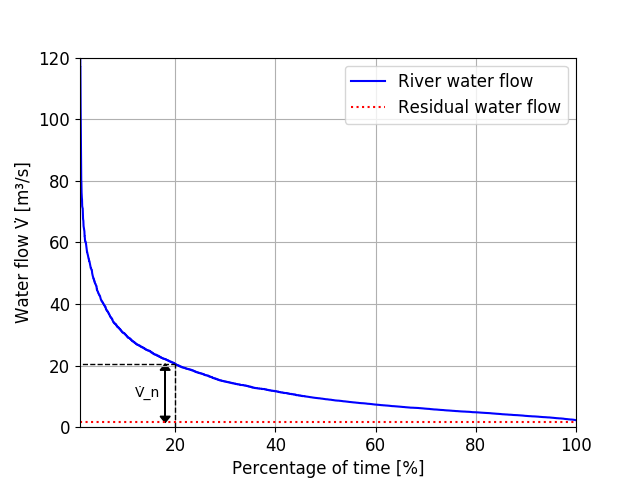
\includegraphics[width=12cm]{fdc.png}
\caption{Extrapolation of nominal water flow from the flow duration curve}
\label{fdc}
\end{figure}

\subsection{Method get{\_}turb{\_}type()}
\label{sub:get_type}

Once the residual water flow and the nominal water flow, head and power are set, the type of turbine can be worked out from locating the turbine on a h\textsubscript{n}/\.{V}\textsubscript{n} diagram such as the one shown on Fig. \ref{charac_diag}. \newline The implementation of this method in Python requires to be able of finding out if a point is inside a polygon. In that effect, a ray casting algorithm was used. Ray casting algorithms use the fact that a point is inside a polygon if a half-line starting from this point intersects the edges of the polygon an uneven number of times.\newline The intersection of half-lines with a polygon edges is not clear in the case where the origin of the half line is on an edge or vertex of the polygon. In our situation, this is automatically counted as being inside the polygon, and the ray casting algorithm is only used for points not locaed on the perimeter of the polygon. \newline To implement a ray casting algorithm in Python, the characteristic diagrams of each turbine type were stored in a csv file by the coordinates of their vertices (see App. \ref{app:csv_vertices}), and a function to test the intersection of two segments was defined as follows : \newline
Segments [AD] and [BC] intersect $\iff 
\left\{
\begin{tabular}{@{}l@{}}
    A and D are on opposite sides of [BC] \\
    AND\\
    B and C are on opposite sides of [AD]
\end{tabular}\right.$\newline
A and D are on opposite sides of [BC] $\iff$ ccw(A,B,C) $\neq$ ccw(D,B,C) \cite{erickson} \newline \\
Where ccw(A,B,C) is a function testing whether A, B and C are in counterclockwise order. \newline  Therefore, testing in [AD] and [BC] intersect is equivalent to testing if only one and only one triplet among \{A,B,C\} and \{D,B,C\} is in counterclockwise order, and if one and only one triplet among \{B,A,D\} and \{C,A,D\} is in counterclockwise order.\newline \\
To test if a triplet \{A,B,C\} of non aligned points is in counterclockwise order, we compute the determinant of $\overrightarrow{AB}$ and $\overrightarrow{BC}$ :\newline
ccw(A,B,C) \tabto{2.5cm}$\iff \mathrm{det}(\overrightarrow{AB},\overrightarrow{AC})>0$\newline \\
\tabto{2.5cm}$\iff \begin{vmatrix}x_B-x_A&x_c-x_A\\y_B-y_A&y_c-y_A\end{vmatrix}>0$\newline\\
\tabto{2.5cm}$\iff (y_C-y_A)\cdot(x_B-x_A) > (y_B-y_A)\cdot(x_C-x_A)$ \newline
Where A, B and C are located by their abscissa x and ordinate y. \newline
\\
Having implemented these two functions in Python, the main function takes a horizontal ray starting in the point (dV\textsubscript{n},h\textsubscript{n}) representing the turbine to test and counts how many time it intersects the edges of each turbine type. When a turbine type gives a uneven number of intersections, the function stops and returns this type. Therefore, in the case of overlapping diagrams, the assignment is made to the first type tested, i.e. to the first type defined in the csv file. In the default file the order is as follows : first Kaplan, then Francis, then Pelton. If no results are found after testing all turbine types defined in the csv file, the function returns the type 'dummy', which represents a virtual turbine. The python script of this method is given in App. \ref{app:get_turb_type}.

\subsection{Calculate power output}

Calling the run{\_}model() method of a Modelchain object calculates the electrical production time series of the plant and stores it in the power{\_}output attribute of the HydropowerPlant object. The run{\_}model() method calls an external function power{\_}output.run() which takes as inputs the HydropowerPlant object, the water flow in the turbine(s) \.{V}-\.{V}\textsubscript{res} and the name of a csv file storing the parameters to calculate the turbine efficiency. If not specified otherwise, a default file is called using parameters from Quaschning \cite{quaschning} listed in Tab. \ref{eff_param} page \ref{eff_param}, and specifying parameters for a ``dummy'' turbine type with a mean efficiency curve. The contents of the csv file are given in App. \ref{app:csv_eff}. \newline
For each timestep of the inflow DataFrame, the load is calculated with Eq. \eqref{eq_load}, the efficiencies of the turbine and generator are calculated based on the values given in Sec. \ref{eff_turb_gen} and an electric power value is calculated from Eq. \eqref{eq_pow}. The flowchart of the function calculating power output is given in Fig. \ref{powout} and the script in App. \ref{app:powout}.
\begin{equation}
 \label{eq_load}
 load = \frac{\dot{V}}{\dot{V}_\mathrm{n}}
\end{equation}

\begin{equation}
  \label{eq_pow}
P= \left\{
    \begin{array}{ll}
	0 & \mbox{if load < turbine minimal load}\\
        P_\mathrm{n} & \mbox{if load}\geq 1 \\
        \eta_\mathrm{turbine} \cdot \eta_\mathrm{generator} \cdot \dot{V} \cdot h_\mathrm{n} \cdot g \cdot \rho & \mbox{otherwise}\\
    \end{array}
\right.
\end{equation}

\begin{figure}[H]
\centering
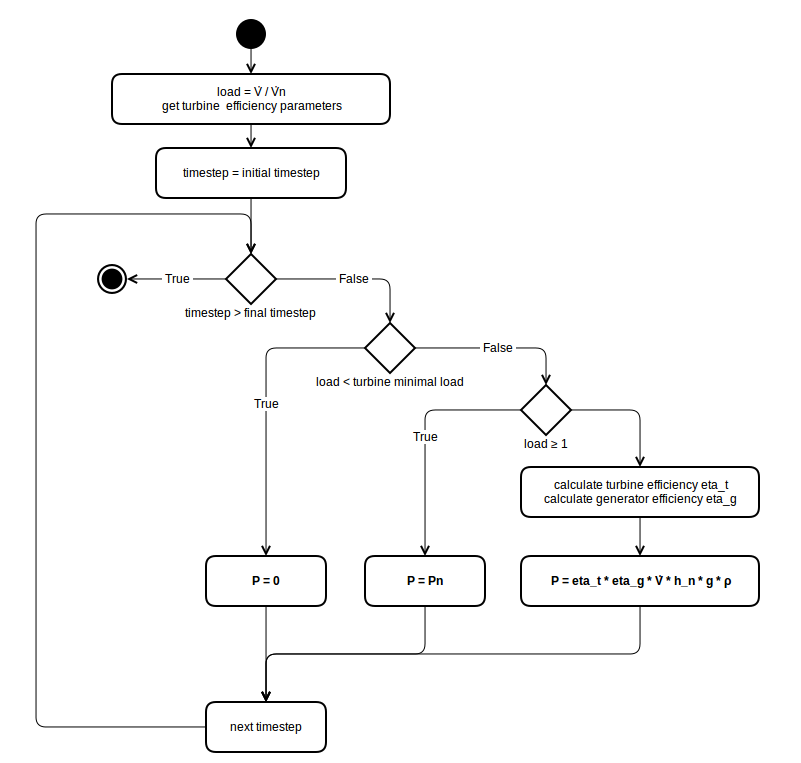
\includegraphics[width=12cm]{powout.png}
\caption{Flowchart of the function calculating the power output}
\label{powout}
\end{figure}



\section{Use examples}
Two use examples are provided with the model to help the user start simulations. Example \ref{sub:ex_with_csv} is designed for simulations with the user's own data (runoff and power plant parameters) and is the study case which results are presented in Sec. \ref{sec:res_single}. Example \ref{sub:ex_with_oedb} is designed for simulations with the OpenEnergy Database and is the study case which results are presented in Sec. \ref{sec:res_th}.

\subsection{With csv files}
\label{sub:ex_with_csv}

This use example aims at simulating the production of a single power plant whose parameters are set by the user, with runoff time series imported from csv files. It is based on a power plant located in the french Vosges, on the Meurthe river. \newline
The first step is to read the runoff time series (historical and over the period to simulate) from csv files and store them into pandas DataFrames with a DateTime index and a column 'dV'.
In this example, the time series over the period to simulate have an hourly timestep and the historical time series have a daily timestep. An instance of the class HydropowerPlant is created, with user defined parameters, and taken as input in an instance of the class Modelchain, along with the runoff time series. \newline
After initialization, the plant parameters are displayed and the simulation can start by calling the run{\_}model() method. The example shows how the production from a single month can be extracted from the output and how the power output can be plotted as a function of time. The code of this example is given in App. \ref{app:ex_with_csv}.

\subsection{With the OpenEnergy Database}
\label{sub:ex_with_oedb}

This use example aims at simulating the production of a region over a year, based on a register of run-of-the-river plants of the region, with runoff time series stored in a database. It is based on power plants of Thuringia and modeled runoff data from the WaterGAP software. The process would be similar with measured runoff data, as long as the database registers have been preprocessed following the guidelines of Sec. \ref{sec:data_preproc}. \newline
The power plant register is imported from the OEDB via a SQL query and a database connection. It is stored in a DataFrame with the plant id, its electrical capacity and the id of the raster cell containing the runoff modeled data. The example iterates over each plant, fetches the available runoff time series from the database, creates HydropowerPlant and Modelchain instances, and stores the power output and parameters of each plant in a DataFrame. \newline
The example counts how many power plants were simulated and displays it, along with the total energy production. The dataframe of plants and power outputs can be exported as csv.The code of this example is given in App. \ref{app:ex_with_oedb}.

	\chapter{Results}
\label{chap:results}
\section{Production prevision for a single turbine}
\label{sec:res_single}
Check on HydroRaon (Ercisol) \newline
Explain the differences in output


\section{Extrapolation of power plant data}
\label{missing_data}
Mosel : check that from Pnenn and flow values over several years we get Hn, Qn and turbine type

\section{Production prevision for a region}
Thüringen cf part methodology on registers
	\chapter{Discussion}

\section{Applications of the model}
\section{Limits}
Good results not possible with gauge stations data because too far from station ? \newline
Will have to be tested again with simulated data from ???

	\chapter{Conclusion}

The objective of this work was to develop with Python an open source model of run-of-the-river hydroelectric power plants able to simulate energy generation time series from open access geodatabases. In particular, the model was to be able to run simulations based on the Open Energy Database, to be consistent with the rest of the work carried out by the ``Transformation of Energy Systems'' team of the Reiner Lemoine Institute. \newline
The choice made in this work was to base the model on the typical equation of hydropower (Eq. \eqref{eq_power_1}) and to extrapolate where necessary missing data about the plants by integrating the steps of the design process for a run-of-the-river plant into the model (Sec. \ref{sub:assumptions}). Thereby, the nominal and residual water flows can be calculated from the flow duration curve on the site of the plant, and an optimal turbine type can be chosen from the nominal head and water flow. In this light, the model meets its basic requirements: it is freely available on github, along with use examples to facilitate the first steps of the user (Ch. \ref{chap:simulation_model}), it does not require more precise data on power plants than what is available in the OEDB, and it produces feed-in time series from hydropower plants. Additionally, the proper way to store runoff data in the OEDB has been discussed and implemented, along with the preprocessing of this data and of the plants registers, in order to assign each plant with consistent runoff time series (Sec. \ref{sec:data_preproc}). \newline
However, the simulations run with this model did not give satisfactory results yet (Ch. \ref{chap:results}). This is due in part to the lack of comprehensive and consistent data to compare with the results, as discussed in Sec. \ref{sec:db_hydroelec}, and in part to the simplifications made in the model and to the assignment of runoff time series to plants. The problems causing the uncertainties have been identified in Sec. \ref{sec:limits} and workarounds have been suggested in Sec. \ref{sec:improv}. \\ 

This project will continue within the openFRED project of the Reiner Lemoine Institute in order to improve the results of the model. The suggestions made in Sec. \ref{sec:improv} can be used to obtain a more precise output. Later on, when the open source modelled runoff data is made available, it will be uploaded into the OEDB and the use examples and preprocessing steps will be adapted to work with this data.\newline
One of the main problems while assessing the quality of the results was the very limited availability of production data from run-of-the-river power plants. It would be extremely interesting for the next steps of the project to have access to production time series of single plants with daily or hourly timesteps, as well as yearly state-wide production specifically from run-of-the-rivers plants. Concerning power plants registers, the publication of the Marktstammdatenregister in the months to come will hopefully provide more precise and comprehensive inputs for the model.


	%% hier eigentliche Kapitel einfügen


	% Anhang
	\appendix
\chapter{Source code}
\label{app:source_code}

\lstinputlisting[caption={Source code}, label=lst:source_code]
	{./data/test.txt}
	%%%%%%%%%%%%%%%%%%%%%%%%%%%%%%%%%%%%%%%%%%%%%%%%%%%%%%%%%%%%%%%%%%%%%%%%%%%%%%%%


	% Literaturverzeichnis
	% Preambel für das Literaturverzeichnis
	\setbibpreamble{The bibliography is sorted alphabetically based on the authors names. In the case of several authors, the work is sorted based on the first author.  \par\bigskip}
	\bibliography{./bibliography/verzeichnis.bib}{} % Datei
	% Layout
	\bibliographystyle{plain}
	% alle Literaturangaben (auch unzitierte)
	\nocite{*}
	% Info: Autoren mit AND trennen, wenn genaue Formatierung ohne Umsortierung gewünscht dann ...= "{...}"
	%%%%%%%%%%%%%%%%%%%%%%%%%%%%%%%%%%%%%%%%%%%%%%%%%%%%%%%%%%%%%%%%%%%%%%%%%%%%%%%%

% Dokumentende
\end{document}
